\documentclass[11pt, journal, onecolumn]{IEEEtran}

\usepackage[utf8]{inputenc}
\usepackage[T1]{fontenc}
\usepackage[english]{babel}
\usepackage{lmodern}
\usepackage{microtype}
\usepackage{amsmath, amssymb, amsthm, mathtools, bm}
\newtheorem{lemma}{Lemma}
\newtheorem{theorem}{Theorem}
\newtheorem{proposition}{Proposition}
\usepackage{siunitx}
\sisetup{locale = US, detect-all = true, exponent-product = \cdot}
\usepackage{booktabs, array, tabularx, multirow, makecell, colortbl}
\usepackage{graphicx}
\graphicspath{{figuras/}}
\usepackage{tikz}
\usetikzlibrary{arrows.meta, positioning, calc, shapes.geometric}
\usepackage{algorithm}
\usepackage{algpseudocode}
\usepackage{cite}
\usepackage{hyperref}
\usepackage{xr-hyper}
\hypersetup{colorlinks=true, linkcolor=blue, citecolor=blue, urlcolor=blue}
\externaldocument[full-]{../auxiliares/SENI142_IEEE_1col}
\makeatletter
\newcommand{\seniSetupExternalRefs}{%
  \let\seni@localref\ref
  \renewcommand{\ref}[1]{\@ifundefined{r@##1}{\seni@localref{full-##1}}{\seni@localref{##1}}}%
}
\makeatother
\AddToHook{begindocument/end}{\seniSetupExternalRefs}

%% --- Paleta cromática institucional SENI-IA ---
\definecolor{seni-blue}{RGB}{0,45,98}
\definecolor{seni-red}{RGB}{206,17,38}
\definecolor{seni-gold}{RGB}{201,168,76}
\definecolor{seni-green}{RGB}{0,122,51}
\definecolor{seni-dark}{RGB}{26,26,26}

\title{SENI-142: Section II — Complete Methodology\\Diakoptic HBCF Schur Formulation and Fail-Closed Digital-Twin Lifecycle}

\author{Junior~Alexis~Villanueva-Rosario,~\IEEEmembership{Ms.C., Ph.D.(c)}\\[0.3em]
{\normalsize\textnormal{\textbf{V-TECH} \textbar\ \textbf{V-CORE TECH S.R.L.} / \textbf{Villa-Core Technologies, S.L.}}}\\[0.15em]
{\footnotesize\textnormal{\textit{Department of Electrical Grids and Renewable Energy (EERR) Research}}}\\[0.15em]
{\footnotesize\textnormal{\textit{Doctoral Chair in Power Systems and Artificial Intelligence}}}\\[0.15em]
{\footnotesize\textnormal{Santo Domingo, Dominican Republic \textbar\ \texttt{ingjavillanueva@gmail.com}}}%
\thanks{J. A. Villanueva-Rosario is with the Department of Electrical Grids and Renewable Energy (EERR) Research, V-TECH (V-CORE TECH S.R.L. / Villa-Core Technologies, S.L.), Santo Domingo, Dominican Republic (e-mail: ingjavillanueva@gmail.com).}}

\renewcommand{\topfraction}{0.95}
\renewcommand{\bottomfraction}{0.95}
\renewcommand{\textfraction}{0.05}
\renewcommand{\floatpagefraction}{0.8}

\begin{document}
\maketitle

\begin{abstract}
This paper introduces SENI-142, an open, fully georeferenced benchmark of the complete bulk transmission system of the Dominican Republic. The model comprises 142 nodal compute buses derived from 112 bulk transmission substations (115 bulk buses at 345, 230, and 138\,kV plus 27 condensed boundary ports at 69\,kV), 135 transmission lines, and 58 power transformers at the 345, 230, and 138\,kV levels; the radial 69\,kV subtransmission layer is condensed into multiport equivalents preserving complex boundary injections and short-circuit impedances. The network is partitioned into ten planning regions aligned with national Law 368-22 and aggregated into four electrical macro-domains. A hierarchical boundary-coordinate formulation (HBCF) is applied, wherein the linear systems arising at each Newton--Raphson iteration are condensed exactly via the Schur complement. On commodity 8-thread hardware, the partitioned solver achieves a full AC state solution in a measured wall-clock time of 2.65\,ms (resident set: 473\,MiB) with an algebraic domain-decomposition residual of $\delta = 2.788 \times 10^{-14}$\,pu relative to a monolithic reference. The structural model is validated across 87\,360 consecutive hourly states (2016--2025) using a 24-hour block bootstrap and evaluated under an official $N-1$ catalogue of 215 contingencies under explicit post-contingency reserve redispatch and bounded slack injection. Multitemporal AC optimal power flow is formulated with power-to-gas, pumped-storage hydro, and biomethanation balances. The dataset, network parameters, and open validation harness are released through IEEE DataPort and a public repository.
\end{abstract}

\begin{IEEEkeywords}
AC-OPF, benchmark testing, diakoptics, digital twins, energy storage, hydrogen, Law 368-22, power system resilience, Schur complement, spatial planning.
\end{IEEEkeywords}

\vspace{10pt}

% =========================================================================
% sec02_methodology_seni_ia.tex — Section II of the sealed master
% sealed master paper_seni142_ieee_transactions_en.md; editorial injection pass 2026-10-17.
% Methodology expansion 2026-10-18: stages 0--7 grafted under the pinned title.
% =========================================================================
\section{Methodology: Diakoptic HBCF Schur Formulation and Fail-Closed Digital-Twin Lifecycle}
\label{sec:methodology}

The methodology is deliberately organized in two coupled components. The \textbf{invariant formulation} --- graph representation, equivalent reduction, spatial partition, exact condensation, data protocol, deterministic lifecycle, regularization, and optimization --- is problem-independent and transfers without modification across the family of studies built on this platform. The \textbf{territorial instantiation clause} binds this formulation to one reference reality: the national grid of the Dominican Republic, partitioned according to the country's own spatial planning statute. This division makes the benchmark a reusable scientific instrument. The subsections below follow that formulation through the numerical pipeline: sealed intake, columnar persistence, nodal physics and reduction, the four-block Jacobian, multi-tier numerical verification, the contingency battery, diakoptic condensation, the three network states, and SHA-512 custody.

\subsection{Steady-State AC Feasibility Scope}
\label{sub:scope}

SENI-142 is strictly a steady-state AC feasibility benchmark. Each solved state is an algebraic equilibrium $F(\mathbf{x})=\mathbf{0}$ on the transmission network. It is an operating point, and the formulation does not integrate a time trajectory. The formulation explicitly does not simulate fast electromagnetic transients (EMT), frequency dynamics, synthetic inertia, rate of change of frequency (RoCoF), frequency nadir, or the actuation of under-frequency load shedding (UFLS/EDAC). The outage of the largest generation block, Punta Catalina (752~MW, about 21.8\% of the 3,450~MW reference national peak demand documented in Table~\ref{tab:regbalance}), is evaluated solely in terms of steady-state voltage margins and post-contingency thermal branch solvability under co-optimized spinning reserve; in the dynamic plane it is a frequency-stability event outside the static frontier of this article.

\subsection{Sealed intake, physical census, and normative screen}
\label{sub:intake}

The solver does not accept a loose file. Entry is a sealed input manifest whose digest is checked before any bus is instantiated, and the manifest selects the physical case. In the measured-estate mode, prospective technologies that are not in commercial operation remain outside the solved dispatch, so the base case is the Dominican system as operated. In the full doctoral-scenario mode those prospective assets may be instantiated; they stay labeled and are never mixed silently into the measured record.

The physical census is the single-line survey already consolidated in Table~\ref{tab:parameters}: the benchmark comprises 142 nodal compute buses derived from 112 bulk transmission substations (115 bulk buses at 345, 230, and 138~kV plus 27 condensed boundary ports at 69~kV), coupled by 135 transmission lines and 58 power transformers. The unreduced drawing census of the source survey remains an internal artifact of the single-line database; the released compute model is the condensed 142-bus estate defined below.

Before any admittance is assembled, a normative screen rejects a record that violates IEEE C37 substation arity or the CIM exchange constraints of IEC 61970 \cite{iec61970}. Series reactances must satisfy $X > 0$, shunt susceptances $B \ge 0$, and two-winding and three-winding transformers must close their own balance. A record that fails the screen aborts the case. It is not repaired by a default.

The same screen is a homologation against current commercial catalogs, not a syntactic patch. Series reactance $X>0$, shunt susceptance $B\ge 0$, and the thermal rating $I_{\max}$ are taken from the catalogs of ACSR and AAAC conductors, of power transformers, and of reactive compensation banks rated up to 250~MVAr. Bay arity and protection classes follow IEEE C37. The exchanged network object follows IEC 61970 (CIM) \cite{iec61970}. None of these values is a synthetic default: a catalog field that fails the screen aborts the case.


\subsection{Columnar persistence and merit-order dispatch}
\label{sub:columnar}

Validated records are laid out as contiguous in-memory columns so that one instruction stream operates on many nodal quantities without copying each record into a relational frame. The layout is an architectural role. On those columns the thermal fleet is ordered by heat-rate merit, and each hour supplies the nodal demand pair $(P_d, Q_d)$ that later enters the power balance.

\subsection{Graph-theoretic representation of the bulk network}
\label{sub:graph}

The transmission system is modeled as a connected undirected graph $\mathcal{G} = (\mathcal{V}, \mathcal{E})$ \cite{newman2010}, where $\mathcal{V}$ is the set of transmission buses ($|\mathcal{V}| = 142$) and $\mathcal{E} = \mathcal{E}_{\mathrm{line}} \cup \mathcal{E}_{\mathrm{trafo}}$ is the union of line and transformer branches, with $|\mathcal{E}_{\mathrm{line}}| = 135$ transmission lines and $|\mathcal{E}_{\mathrm{trafo}}| = 58$ power transformers. Each branch carries a per-unit series admittance and half-charging susceptance on a common 100~MVA base; the nodal admittance matrix $\mathbf{Y}_{\mathrm{bus}} \in \mathbb{C}^{142 \times 142}$ therefore encodes 20,164 complex entries of coupled electromagnetic state. Nodal power injections follow the standard rectangular balance
\begin{equation}
S_i = P_i + jQ_i = V_i \sum_{j \in \mathcal{V}} Y_{ij}^{*}\, V_j^{*}, \qquad i \in \mathcal{V},
\label{eq:balance}
\end{equation}
with buses classified as slack, PV, or PQ \cite{tinney1967}. The angle reference is the 345~kV bus of the Julio Sauri substation (JSAURI), held at $V = 1.02\ \mathrm{pu}$. Its active power is the bounded variable of \eqref{eq:slackbox} and is not an unbounded mismatch reservoir. That bus receives directly the injection of the largest thermal plant in the country (Section~\ref{sub:strata}). Where a physical substation hosts more than one voltage level, each voltage level is a distinct bus and the intervening autotransformer is a branch. The reconciliation of Section~\ref{sub:crosswalk} is what carries the 112 bulk transmission substations to the 142 nodal compute buses (115 bulk buses at 345, 230, and 138~kV plus 27 condensed boundary ports at 69~kV; Section~\ref{sub:substations}).

Figure~\ref{fig:topologia142} places the 142 solved nodes in the four electrical macrodomains of Law 368-22 ($\Omega_1$ Norte, $\Omega_2$ Sur, $\Omega_3$ Este, $\Omega_4$ Metropolitano). Bulk yards keep the color of their measured nominal voltage, 345~kV, 230~kV, or 138~kV. The 27 retained boundary terminals stay at the measured 69~kV and are drawn in green. The compute model counts 135 transmission lines. The figure draws a stroke for each pair the census closes: a yard record that names both terminals, or a colinear one-line trace that arrives at a second solved bus of the same voltage. A record whose far terminal is not a census bus is omitted.

% Full-page schematic of the 142-node trunk.
% 115 named bulk yards plus 27 retained 69 kV boundary terminals.
% Panel schematic. Raw drawing coordinates are not printed.

\begin{figure*}[!p]
\centering
\resizebox{\textwidth}{0.80\textheight}{%
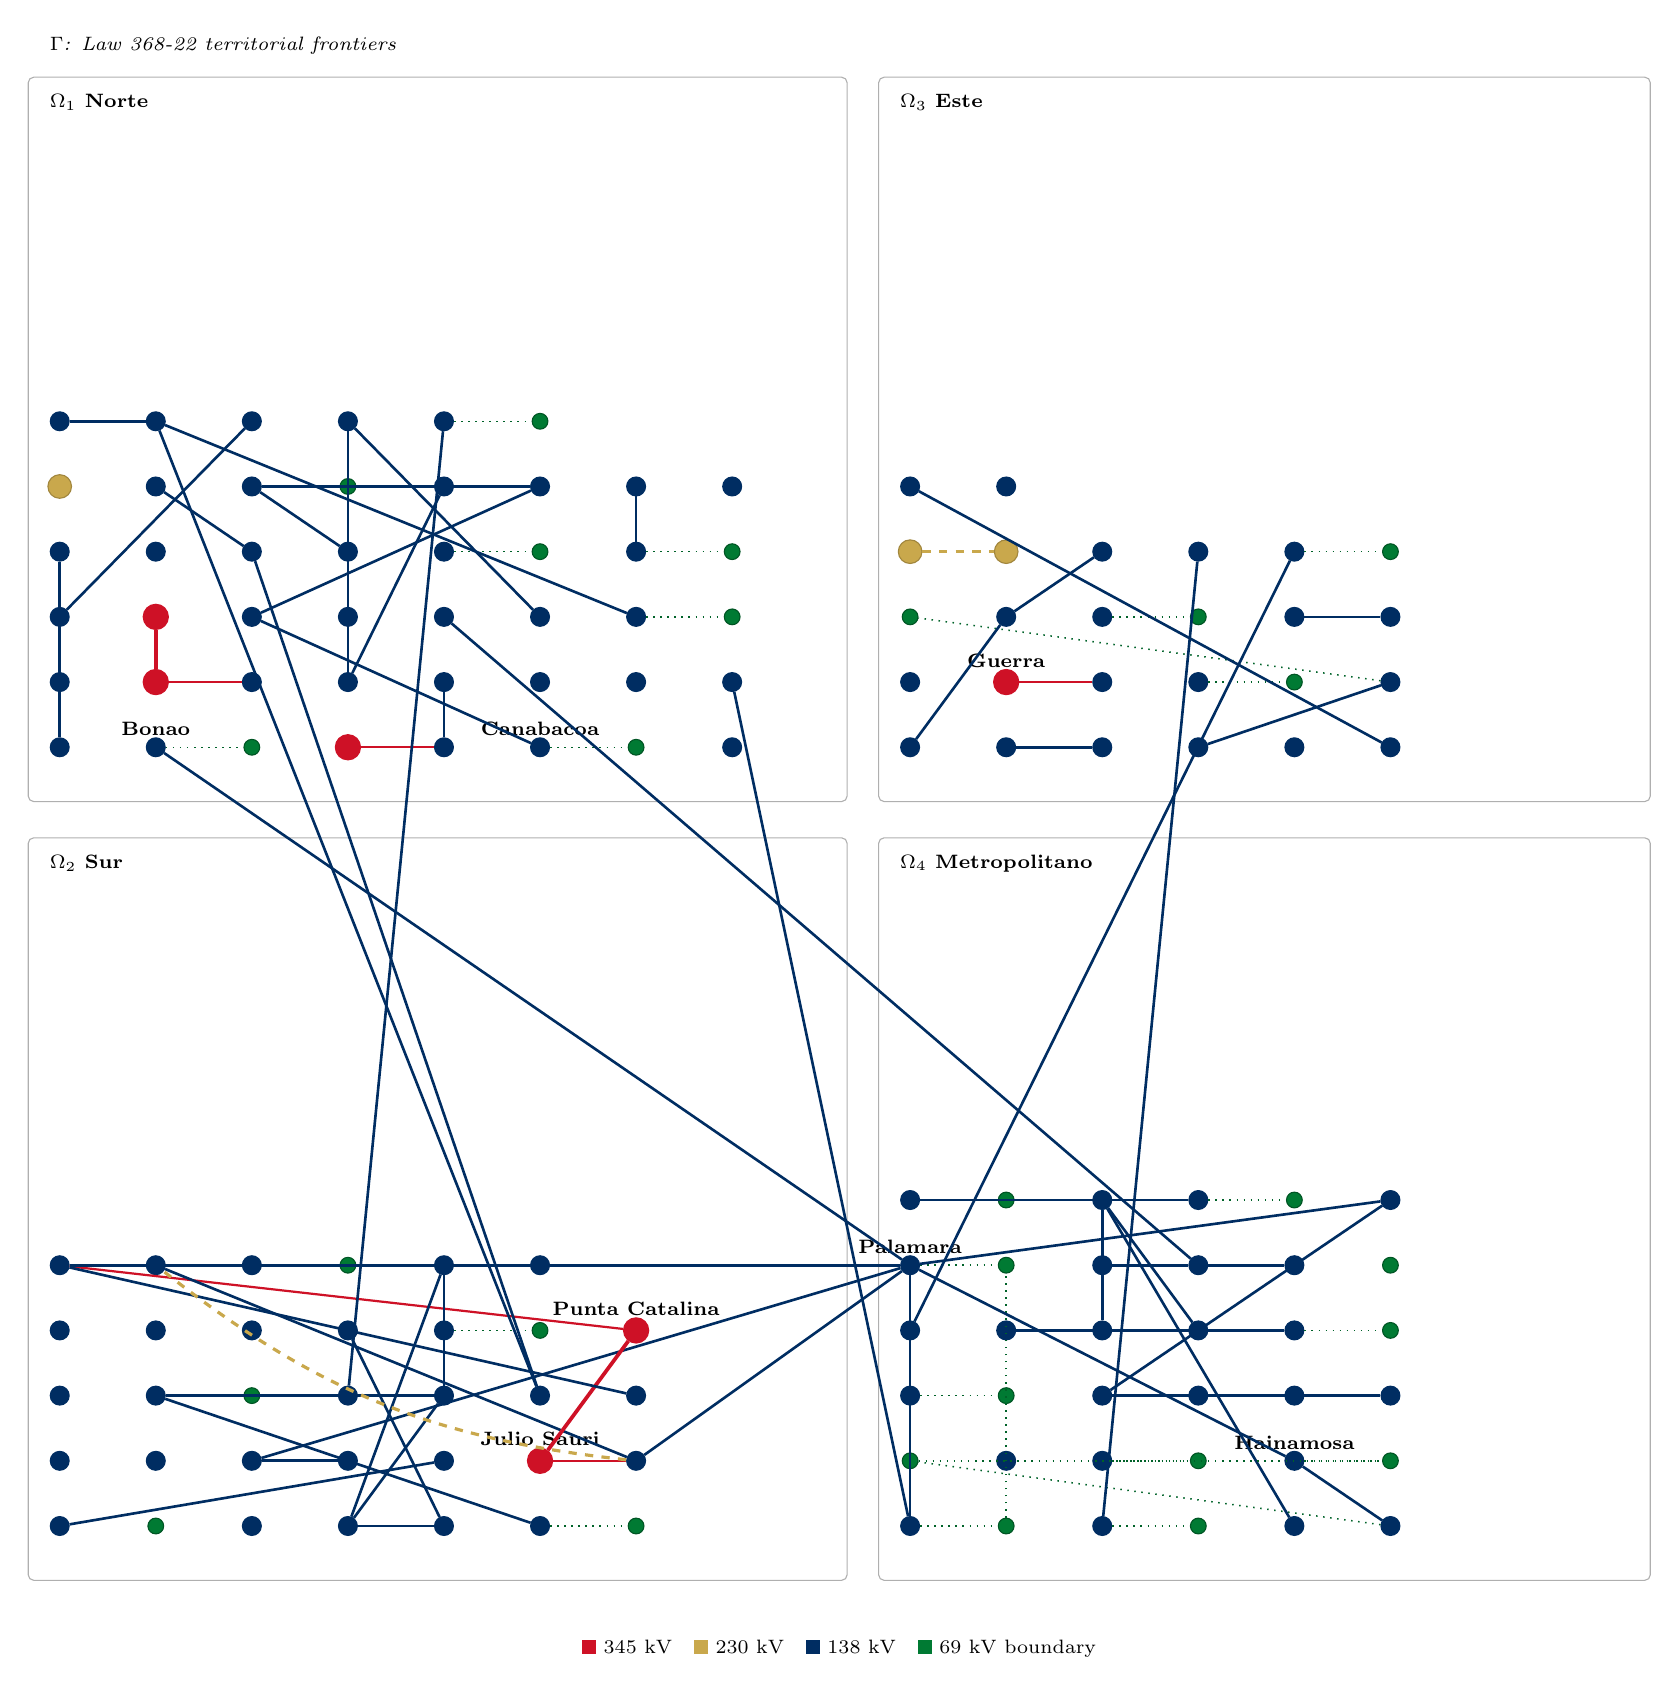
\begin{tikzpicture}[x=1cm,y=1.15cm,
  bus345/.style={circle, fill=seni-red, draw=seni-red, inner sep=0pt, minimum size=3.2mm},
  bus230/.style={circle, fill=seni-gold, draw=seni-gold!80!black, inner sep=0pt, minimum size=3.0mm},
  bus138/.style={circle, fill=seni-blue, draw=seni-blue, inner sep=0pt, minimum size=2.4mm},
  bus69/.style={circle, fill=seni-green, draw=seni-green!70!black, inner sep=0pt, minimum size=2.0mm},
  trunk345/.style={line width=1.35pt, seni-red},
  trunk230/.style={line width=1.15pt, seni-gold, dashed},
  trunk138/.style={line width=0.95pt, seni-blue},
  tie345/.style={line width=0.8pt, seni-red},
  tie230/.style={line width=0.75pt, seni-gold},
  tie138/.style={line width=0.6pt, seni-blue!70},
  tie69/.style={line width=0.55pt, seni-green!80!black, dotted}
]
\draw (0.15,16.95) node[anchor=west, font=\scriptsize\itshape] {$\Gamma$: Law 368-22 territorial frontiers};
\draw (10.3,-0.55) node[anchor=north, font=\scriptsize] {{\color{seni-red}\rule{5pt}{5pt}}~345~kV\quad {\color{seni-gold}\rule{5pt}{5pt}}~230~kV\quad {\color{seni-blue}\rule{5pt}{5pt}}~138~kV\quad {\color{seni-green}\rule{5pt}{5pt}}~69~kV boundary};
\draw[rounded corners=2pt, draw=seni-dark!35] (0.0,8.6) rectangle (10.4,16.6);
\draw (0.15,16.32) node[anchor=west, font=\bfseries\scriptsize] {$\Omega_1$ Norte};
\draw[rounded corners=2pt, draw=seni-dark!35] (10.8,8.6) rectangle (20.6,16.6);
\draw (10.95,16.32) node[anchor=west, font=\bfseries\scriptsize] {$\Omega_3$ Este};
\draw[rounded corners=2pt, draw=seni-dark!35] (0.0,0.0) rectangle (10.4,8.2);
\draw (0.15,7.92) node[anchor=west, font=\bfseries\scriptsize] {$\Omega_2$ Sur};
\draw[rounded corners=2pt, draw=seni-dark!35] (10.8,0.0) rectangle (20.6,8.2);
\draw (10.95,7.92) node[anchor=west, font=\bfseries\scriptsize] {$\Omega_4$ Metropolitano};
\node[bus345] (bBONAO3345) at (4.06,9.2) {};
\node[bus345] (bELNARANJO345) at (1.62,9.92) {};
\node[bus345, label={[font=\scriptsize\bfseries, inner sep=0.4pt]above:Guerra}] (bGUERRA345) at (12.42,9.92) {};
\node[bus345, label={[font=\scriptsize\bfseries, inner sep=0.4pt]above:Julio Sauri}] (bJULIOSAURI345) at (6.5,1.32) {};
\node[bus345] (bMANZANILLOPOWERLAND345) at (1.62,10.64) {};
\node[bus345, label={[font=\scriptsize\bfseries, inner sep=0.4pt]above:Punta Catalina}] (bPUNTACATALINA345) at (7.72,2.76) {};
\node[bus230] (bPVDC230) at (0.4,12.08) {};
\node[bus230] (bQUISQUEYA1230) at (11.2,11.36) {};
\node[bus230] (bQUISQUEYA2230) at (12.42,11.36) {};
\node[bus138] (bSPM138) at (16.08,11.36) {};
\node[bus138] (bSPM2138) at (11.2,12.08) {};
\node[bus138] (bAGUACLARA138) at (0.4,9.2) {};
\node[bus138] (bAGUACATE138) at (0.4,0.6) {};
\node[bus138] (bARROYOHONDO138) at (11.2,0.6) {};
\node[bus138] (bBARAHONACARBON138) at (2.84,0.6) {};
\node[bus138] (bBAYASOL138) at (4.06,0.6) {};
\node[bus138] (bBOCACHICA138) at (13.64,0.6) {};
\node[bus138, label={[font=\scriptsize\bfseries, inner sep=0.4pt]above:Bonao}] (bBONAO2138) at (1.62,9.2) {};
\node[bus138] (bBONAO3138) at (5.28,9.2) {};
\node[bus138] (bCALABAZA138) at (5.28,0.6) {};
\node[bus138, label={[font=\scriptsize\bfseries, inner sep=0.4pt]above:Canabacoa}] (bCANABACOA138) at (6.5,9.2) {};
\node[bus138] (bCIPLALUISA138) at (11.2,9.2) {};
\node[bus138] (bCNP138) at (16.08,0.6) {};
\node[bus138] (bCOASTAL138) at (12.42,9.2) {};
\node[bus138] (bCOTOPERI138) at (8.94,9.2) {};
\node[bus138] (bCRUCEDECABRAL2138) at (6.5,0.6) {};
\node[bus138] (bCUMAYASA138) at (13.64,9.2) {};
\node[bus138] (bDAJABON138) at (0.4,9.92) {};
\node[bus138] (bDAJAO138) at (17.3,0.6) {};
\node[bus138] (bELBRISAL138) at (0.4,1.32) {};
\node[bus138] (bELNARANJO138) at (2.84,9.92) {};
\node[bus138] (bELSEIBO138) at (14.86,9.2) {};
\node[bus138] (bELSOCO138) at (16.08,9.2) {};
\node[bus138] (bEMBAJADOR138) at (12.42,1.32) {};
\node[bus138] (bENERGAS4138) at (17.3,9.2) {};
\node[bus138] (bESPERANZA138) at (4.06,9.92) {};
\node[bus138] (bFALCONDO138) at (5.28,9.92) {};
\node[bus138] (bGIRASOL138) at (11.2,9.92) {};
\node[bus138] (bGUANILLO138) at (6.5,9.92) {};
\node[bus138] (bGUAYUBIN138) at (7.72,9.92) {};
\node[bus138] (bGUERRA138) at (13.64,9.92) {};
\node[bus138] (bGUZMANCITO138) at (1.62,1.32) {};
\node[bus138] (bHAINA138) at (13.64,1.32) {};
\node[bus138, label={[font=\scriptsize\bfseries, inner sep=0.4pt]above:Hainamosa}] (bHAINAMOSA138) at (16.08,1.32) {};
\node[bus138] (bHATOMAYOR2138) at (14.86,9.92) {};
\node[bus138] (bHERRERA138) at (11.2,2.04) {};
\node[bus138] (bHIGUEY138) at (17.3,9.92) {};
\node[bus138] (bITABO138) at (2.84,1.32) {};
\node[bus138] (bITABOTG138) at (4.06,1.32) {};
\node[bus138] (bJIGUEY138) at (5.28,1.32) {};
\node[bus138] (bJIMANI138) at (0.4,2.04) {};
\node[bus138] (bJUANDOLIO138) at (12.42,10.64) {};
\node[bus138] (bJULIOSAURI138) at (7.72,1.32) {};
\node[bus138] (bKM15DEAZUA138) at (1.62,2.04) {};
\node[bus138] (bLAGALLERA138) at (4.06,2.04) {};
\node[bus138] (bLAISABELA138) at (8.94,9.92) {};
\node[bus138] (bLAROMANA138) at (13.64,10.64) {};
\node[bus138] (bLOPEZANGOSTURA138) at (0.4,10.64) {};
\node[bus138] (bLOSMINA138) at (13.64,2.04) {};
\node[bus138] (bLOSMINA5138) at (14.86,2.04) {};
\node[bus138] (bLOSMINA6138) at (16.08,2.04) {};
\node[bus138] (bLOSMINA7138) at (17.3,2.04) {};
\node[bus138] (bLOSORIGENES138) at (11.2,2.76) {};
\node[bus138] (bLOSPRADOS138) at (12.42,2.76) {};
\node[bus138] (bMATADEPALMA2138) at (16.08,10.64) {};
\node[bus138] (bMATADERO138) at (13.64,2.76) {};
\node[bus138] (bMATAFONGO138) at (5.28,2.04) {};
\node[bus138] (bMATRISOL138) at (6.5,2.04) {};
\node[bus138] (bMETALDOM138) at (14.86,2.76) {};
\node[bus138] (bMETROPOLITANO138) at (16.08,2.76) {};
\node[bus138] (bMIRASOL138) at (17.3,10.64) {};
\node[bus138] (bMOCA138) at (2.84,10.64) {};
\node[bus138] (bMONCION138) at (6.5,10.64) {};
\node[bus138] (bMONTECRISTI138) at (4.06,10.64) {};
\node[bus138] (bMONTERIO138) at (5.28,10.64) {};
\node[bus138] (bNAGUA2138) at (7.72,10.64) {};
\node[bus138] (bNAVARRETE2138) at (0.4,11.36) {};
\node[bus138] (bNIBAJE138) at (1.62,11.36) {};
\node[bus138, label={[font=\scriptsize\bfseries, inner sep=0.4pt]above:Palamara}] (bPALAMARA138) at (11.2,3.48) {};
\node[bus138] (bPALENQUE138) at (7.72,2.04) {};
\node[bus138] (bPALOMINO138) at (0.4,2.76) {};
\node[bus138] (bPARAISO138) at (1.62,2.76) {};
\node[bus138] (bPAYITA138) at (2.84,11.36) {};
\node[bus138] (bPEDERNALES138) at (2.84,2.76) {};
\node[bus138] (bPERAVIA138) at (4.06,2.76) {};
\node[bus138] (bPIMENTEL138) at (4.06,11.36) {};
\node[bus138] (bPIZARRETE138) at (5.28,2.76) {};
\node[bus138] (bPLAYADORADA138) at (5.28,11.36) {};
\node[bus138] (bPOWERSHIPKPS01138) at (13.64,3.48) {};
\node[bus138] (bPOWERSHIPKPS26138) at (14.86,3.48) {};
\node[bus138] (bPOWERSHIPKPS60138) at (16.08,3.48) {};
\node[bus138] (bPUERTOPLATA2138) at (7.72,11.36) {};
\node[bus138] (bPUNTACATALINA138) at (0.4,3.48) {};
\node[bus138] (bRIOSANJUAN138) at (1.62,12.08) {};
\node[bus138] (bSFM138) at (2.84,12.08) {};
\node[bus138] (bSAJOMA138) at (5.28,12.08) {};
\node[bus138] (bSALCEDO138) at (6.5,12.08) {};
\node[bus138] (bSAMANA138) at (0.4,12.8) {};
\node[bus138] (bSANCRISTOBALNORTE138) at (1.62,3.48) {};
\node[bus138] (bSANFELIPE138) at (7.72,12.08) {};
\node[bus138] (bSANJUAN2138) at (2.84,3.48) {};
\node[bus138] (bSANPEDROBIOENERGY138) at (13.64,11.36) {};
\node[bus138] (bSANCHEZ138) at (1.62,12.8) {};
\node[bus138] (bSANTANASOL138) at (5.28,3.48) {};
\node[bus138] (bSANTIAGORODRIGUEZ138) at (8.94,12.08) {};
\node[bus138] (bSIBA138) at (14.86,11.36) {};
\node[bus138] (bSULTANADELESTE138) at (12.42,12.08) {};
\node[bus138] (bTAVERA138) at (2.84,12.8) {};
\node[bus138] (bTIMBEQUE2138) at (11.2,4.2) {};
\node[bus138] (bUASD138) at (13.64,4.2) {};
\node[bus138] (bVALDESIA138) at (6.5,3.48) {};
\node[bus138] (bVALVERDEMAO138) at (4.06,12.8) {};
\node[bus138] (bVILLADUARTE138) at (14.86,4.2) {};
\node[bus138] (bVILLAMELLA138) at (17.3,4.2) {};
\node[bus138] (bZFSANTIAGO138) at (5.28,12.8) {};
\node[bus69] (bARROYOHONDO69) at (12.42,0.6) {};
\node[bus69] (bBARAHONA69) at (1.62,0.6) {};
\node[bus69] (bBOCACHICA69) at (14.86,0.6) {};
\node[bus69] (bBONAO269) at (2.84,9.2) {};
\node[bus69] (bCANABACOA69) at (7.72,9.2) {};
\node[bus69] (bCRUCEDECABRAL269) at (7.72,0.6) {};
\node[bus69] (bDAJAO69) at (11.2,1.32) {};
\node[bus69] (bHAINA69) at (14.86,1.32) {};
\node[bus69] (bHAINAMOSA69) at (17.3,1.32) {};
\node[bus69] (bHATOMAYOR269) at (16.08,9.92) {};
\node[bus69] (bHERRERA69) at (12.42,2.04) {};
\node[bus69] (bHIGUEY69) at (11.2,10.64) {};
\node[bus69] (bKM15DEAZUA69) at (2.84,2.04) {};
\node[bus69] (bMETROPOLITANO69) at (17.3,2.76) {};
\node[bus69] (bNAGUA269) at (8.94,10.64) {};
\node[bus69] (bPALAMARA69) at (12.42,3.48) {};
\node[bus69] (bPIZARRETE69) at (6.5,2.76) {};
\node[bus69] (bPLAYADORADA69) at (6.5,11.36) {};
\node[bus69] (bPUERTOPLATA269) at (8.94,11.36) {};
\node[bus69] (bLAROMANA69) at (14.86,10.64) {};
\node[bus69] (bSANJUAN269) at (4.06,3.48) {};
\node[bus69] (bSFM69) at (4.06,12.08) {};
\node[bus69] (bSPM69) at (17.3,11.36) {};
\node[bus69] (bTIMBEQUE69) at (17.3,3.48) {};
\node[bus69] (bTIMBEQUE269) at (12.42,4.2) {};
\node[bus69] (bVILLADUARTE69) at (16.08,4.2) {};
\node[bus69] (bZFSANTIAGO69) at (6.5,12.8) {};
\draw[tie345] (bBONAO3345) -- (bBONAO3138);
\draw[tie345] (bELNARANJO345) -- (bELNARANJO138);
\draw[tie345] (bGUERRA345) -- (bGUERRA138);
\draw[tie345] (bJULIOSAURI345) -- (bJULIOSAURI138);
\draw[tie345] (bPUNTACATALINA345) -- (bPUNTACATALINA138);
\draw[tie69] (bSPM138) -- (bSPM69);
\draw[tie69] (bARROYOHONDO138) -- (bARROYOHONDO69);
\draw[tie69] (bBOCACHICA138) -- (bBOCACHICA69);
\draw[tie69] (bBONAO2138) -- (bBONAO269);
\draw[tie69] (bCANABACOA138) -- (bCANABACOA69);
\draw[tie69] (bCRUCEDECABRAL2138) -- (bCRUCEDECABRAL269);
\draw[tie69] (bDAJAO138) -- (bDAJAO69);
\draw[tie69] (bHAINA138) -- (bHAINA69);
\draw[tie69] (bHAINAMOSA138) -- (bHAINAMOSA69);
\draw[tie69] (bHATOMAYOR2138) -- (bHATOMAYOR269);
\draw[tie69] (bHERRERA138) -- (bHERRERA69);
\draw[tie69] (bHIGUEY138) -- (bHIGUEY69);
\draw[tie69] (bKM15DEAZUA138) -- (bKM15DEAZUA69);
\draw[tie69] (bLAROMANA138) -- (bLAROMANA69);
\draw[tie69] (bMETROPOLITANO138) -- (bMETROPOLITANO69);
\draw[tie69] (bNAGUA2138) -- (bNAGUA269);
\draw[tie69] (bPALAMARA138) -- (bPALAMARA69);
\draw[tie69] (bPIZARRETE138) -- (bPIZARRETE69);
\draw[tie69] (bPLAYADORADA138) -- (bPLAYADORADA69);
\draw[tie69] (bPUERTOPLATA2138) -- (bPUERTOPLATA269);
\draw[tie69] (bSFM138) -- (bSFM69);
\draw[tie69] (bSANJUAN2138) -- (bSANJUAN269);
\draw[tie69] (bTIMBEQUE2138) -- (bTIMBEQUE269);
\draw[tie69] (bVILLADUARTE138) -- (bVILLADUARTE69);
\draw[tie69] (bZFSANTIAGO138) -- (bZFSANTIAGO69);
\draw[trunk138] (bAGUACLARA138) -- (bNAVARRETE2138);
\draw[trunk138] (bAGUACATE138) -- (bJIGUEY138);
\draw[tie69] (bARROYOHONDO69) -- (bPALAMARA69);
\draw[trunk138] (bARROYOHONDO138) -- (bLAISABELA138);
\draw[trunk138] (bARROYOHONDO138) -- (bPALAMARA138);
\draw[trunk138] (bBAYASOL138) -- (bCALABAZA138);
\draw[trunk138] (bBAYASOL138) -- (bMATAFONGO138);
\draw[trunk138] (bBAYASOL138) -- (bSANTANASOL138);
\draw[trunk138] (bBOCACHICA138) -- (bSIBA138);
\draw[trunk138] (bBONAO2138) -- (bPALAMARA138);
\draw[trunk138] (bBONAO3138) -- (bFALCONDO138);
\draw[trunk138] (bCALABAZA138) -- (bPERAVIA138);
\draw[trunk138] (bCANABACOA138) -- (bMOCA138);
\draw[trunk138] (bCIPLALUISA138) -- (bJUANDOLIO138);
\draw[trunk138] (bCNP138) -- (bUASD138);
\draw[trunk138] (bCOASTAL138) -- (bCUMAYASA138);
\draw[trunk138] (bCRUCEDECABRAL2138) -- (bKM15DEAZUA138);
\draw[tie69] (bDAJAO69) -- (bHAINAMOSA69);
\draw[trunk138] (bDAJAO138) -- (bHAINAMOSA138);
\draw[trunk345] (bELNARANJO345) -- (bMANZANILLOPOWERLAND345);
\draw[trunk138] (bELSEIBO138) -- (bHIGUEY138);
\draw[trunk138] (bENERGAS4138) -- (bSPM2138);
\draw[trunk138] (bESPERANZA138) -- (bSAJOMA138);
\draw[trunk138] (bESPERANZA138) -- (bVALVERDEMAO138);
\draw[trunk138] (bHAINAMOSA138) -- (bPALAMARA138);
\draw[trunk138] (bITABO138) -- (bITABOTG138);
\draw[trunk138] (bITABO138) -- (bPALAMARA138);
\draw[trunk138] (bJUANDOLIO138) -- (bSANPEDROBIOENERGY138);
\draw[trunk138] (bJULIOSAURI138) -- (bPALAMARA138);
\draw[trunk138] (bJULIOSAURI138) -- (bSANCRISTOBALNORTE138);
\draw[trunk345] (bJULIOSAURI345) -- (bPUNTACATALINA345);
\draw[trunk138] (bKM15DEAZUA138) -- (bMATAFONGO138);
\draw[trunk138] (bLAGALLERA138) -- (bZFSANTIAGO138);
\draw[trunk138] (bLOPEZANGOSTURA138) -- (bTAVERA138);
\draw[trunk138] (bLOSMINA138) -- (bLOSMINA5138);
\draw[trunk138] (bLOSMINA138) -- (bLOSMINA6138);
\draw[trunk138] (bLOSMINA138) -- (bLOSMINA7138);
\draw[trunk138] (bLOSMINA138) -- (bVILLAMELLA138);
\draw[trunk138] (bLOSMINA5138) -- (bLOSMINA6138);
\draw[trunk138] (bLOSMINA6138) -- (bLOSMINA7138);
\draw[trunk138] (bLOSORIGENES138) -- (bSPM138);
\draw[trunk138] (bLOSPRADOS138) -- (bMETROPOLITANO138);
\draw[trunk138] (bMATADEPALMA2138) -- (bMIRASOL138);
\draw[trunk138] (bMATADERO138) -- (bMETALDOM138);
\draw[trunk138] (bMATADERO138) -- (bUASD138);
\draw[trunk138] (bMATAFONGO138) -- (bPIZARRETE138);
\draw[trunk138] (bMATAFONGO138) -- (bSANTANASOL138);
\draw[trunk138] (bMATRISOL138) -- (bPAYITA138);
\draw[trunk138] (bMATRISOL138) -- (bSANCHEZ138);
\draw[trunk138] (bMETALDOM138) -- (bUASD138);
\draw[trunk138] (bMOCA138) -- (bSALCEDO138);
\draw[trunk138] (bMONCION138) -- (bVALVERDEMAO138);
\draw[trunk138] (bMONTERIO138) -- (bPOWERSHIPKPS26138);
\draw[trunk138] (bNAGUA2138) -- (bSANCHEZ138);
\draw[trunk138] (bPALAMARA138) -- (bSANCRISTOBALNORTE138);
\draw[trunk138] (bPALAMARA138) -- (bVALDESIA138);
\draw[trunk138] (bPALAMARA138) -- (bVILLAMELLA138);
\draw[trunk138] (bPALENQUE138) -- (bPUNTACATALINA138);
\draw[trunk138] (bPAYITA138) -- (bRIOSANJUAN138);
\draw[trunk138] (bPIMENTEL138) -- (bSFM138);
\draw[trunk138] (bPIZARRETE138) -- (bSANTANASOL138);
\draw[trunk138] (bPOWERSHIPKPS01138) -- (bPOWERSHIPKPS26138);
\draw[trunk138] (bPOWERSHIPKPS26138) -- (bPOWERSHIPKPS60138);
\draw[trunk138] (bPUERTOPLATA2138) -- (bSANFELIPE138);
\draw[trunk138] (bPUNTACATALINA138) -- (bVALDESIA138);
\draw[trunk230] (bQUISQUEYA1230) -- (bQUISQUEYA2230);
\draw[trunk138] (bSFM138) -- (bSALCEDO138);
\draw[trunk138] (bSAMANA138) -- (bSANCHEZ138);
\draw[trunk138] (bSANCRISTOBALNORTE138) -- (bVALDESIA138);
\draw[trunk138] (bTIMBEQUE2138) -- (bVILLADUARTE138);
\draw[trunk230] (bJULIOSAURI138) to[bend left=16] (bSANCRISTOBALNORTE138);
\end{tikzpicture}%
}
\caption{Schematic of the 142-node trunk, grouped into the four electrical macrodomains of Law 368-22 ($\Omega_1$ Norte, $\Omega_2$ Sur, $\Omega_3$ Este, $\Omega_4$ Metropolitano). Color is the measured nominal voltage: 345~kV in red, 230~kV in gold, 138~kV in blue, and the 27 retained 69~kV boundary terminals in green. A stroke joins two solved buses only: same-estate autotransformer links; yard records that name both ends, including the Palamara 138~kV bays to Julio Sauri, San Cristobal Norte, Hainamosa, Itabo, Valdesia, Bonao 2, Villa Mella and Arroyo Hondo; the 345~kV corridors Punta Catalina--Julio Sauri and Manzanillo Power Land--El Naranjo; the 138~kV link km~15 de Azua--Cruce de Cabral~2; the 230~kV tie Quisqueya~1--Quisqueya~2; and every other same-voltage pair whose colinear one-line trace arrives at a second census label. Parallel circuits are one stroke. The dashed bent stroke is the published 230~kV Julio Sauri--San Cristobal Norte reinforcement between the two 138~kV estates, because the census declares no separate 230~kV bus there. A record whose far terminal is not a census bus is omitted. Panel positions are schematic. Raw drawing coordinates are not shown.}
\label{fig:topologia142}
\end{figure*}



\subsection{Equivalent reduction of the 69 kV subtransmission layer}
\label{sub:reduction}

Sixty-three radial laterals of the 69~kV layer are condensed into static multiport equivalents of Th\'evenin/Norton type. For each retained boundary terminal, which stays at its measured 69~kV, the equivalent preserves (i) the aggregated complex injection of the condensed area at every modeled hour and (ii) the short-circuit impedance $Z_{\mathrm{cc}}$ seen from that terminal, obtained by Kron-type network reduction. Formally, for boundary port $p$ with condensed interior $\Omega_r$,
\begin{equation}
V_p = E_{\mathrm{th}}^{(r)} - Z_{\mathrm{th}}^{(r)} I_p, \qquad \sum_{i \in \Omega_r} S_i = V_p I_p^{*} + \Delta S_{\mathrm{loss}},
\label{eq:thevenin}
\end{equation}
so that the boundary power balance explicitly accounts for the internal losses represented by $\Delta S_{\mathrm{loss}}$ while the equivalent preserves the retained-port variables and eliminates dimensional inflation of $\mathbf{Y}_{\mathrm{bus}}$. The reduction is recomputed from the archived configuration of the estate and is itself part of the sealed artifact, consistent with recommended practice for industrial system analysis \cite{ieee399} and with CIM-based interchange of network models \cite{iec61970}.

Of the ninety 69~kV busbars, sixty-three are the radial laterals removed above. The other twenty-seven remain solved buses at the measured 69~kV. Each of those twenty-seven is a retained boundary terminal. The 115 bulk nodes of Table~\ref{tab:parameters} are the census buses at 345, 230, and 138~kV. The model that is actually solved has 142 buses: those 115 bulk nodes plus these 27 terminals at 69~kV. Removing the sixty-three laterals is also why a fast-decoupled flow and Gauss--Seidel converge on this estate: the branches whose $R/X$ ratio would otherwise singularize the Jacobian are no longer nodes of the solved system. Synchronous units keep their full $P$--$Q$ capability. Static renewable plants are not synchronous machines; their reactive support is stated with the continuous map of Section~\ref{sub:regularization}.


\subsection{Breadth-first scaling of connectivity}
\label{sub:bfs}

Let $\mathcal{G}_Y=(\mathcal{V},\mathcal{E}_Y)$ be the sparsity graph of $\mathbf{Y}_{\mathrm{bus}}$: an undirected edge exists wherever a retained branch has nonzero admittance. Breadth-first search (BFS), the connectivity scaling denoted M09, starts at the Julio Sauri slack and visits every bus reachable on $\mathcal{G}_Y$. Algorithm~\ref{alg:bfs} is the procedure. A bus that remains unvisited belongs to another connected component. That component is an electrical island: it has no finite power-flow state, and its voltage magnitude is recorded as $V_m=\mathrm{NaN}$ rather than as a fabricated residual. After the traversal, every visited bus of degree one is a radial antenna and is a candidate for the 69~kV condensation of Section~\ref{sub:reduction}. Discovery order then places interior buses before border buses. That order is the permutation applied to the connectivity before the Schur partition of Section~\ref{sub:hbcf}.

\begin{algorithm}[!t]
\caption{Breadth-first scaling on the admittance graph (M09)}
\label{alg:bfs}
\begin{algorithmic}[1]
\Require sparsity graph $\mathcal{G}_Y=(\mathcal{V},\mathcal{E}_Y)$, slack $s$
\State $Q \gets (s)$, $\mathrm{seen}\gets\{s\}$, $\pi\gets(s)$
\While{$Q\neq\emptyset$}
  \State $u \gets \mathrm{pop}(Q)$
  \For{$v\in\mathcal{N}(u)$}
    \If{$v\notin\mathrm{seen}$}
      \State $\mathrm{seen}\gets\mathrm{seen}\cup\{v\}$; append $v$ to $Q$ and to $\pi$
    \EndIf
  \EndFor
\EndWhile
\State $\mathcal{I}\gets\mathcal{V}\setminus\mathrm{seen}$ \Comment{islands, $V_m=\mathrm{NaN}$}
\State $\mathcal{A}\gets\{u\in\mathrm{seen}:\deg(u)=1\}$ \Comment{radial antennas}
\State \Return permutation $\pi$, islands $\mathcal{I}$, antennas $\mathcal{A}$
\end{algorithmic}
\end{algorithm}

The reordering is a permutation matrix $\mathbf{P}$. Singular values are invariant under permutation similarity, so $\kappa_2(\mathbf{P}\mathbf{J}\mathbf{P}^{T})=\kappa_2(\mathbf{J})$. The BFS itself does not move the condition number and does not enlarge the state dimension. On the SENI-RD base case the measured movement is a change of operating point between the real network and the ideal network:
\begin{equation}
\begin{aligned}
\kappa_{\mathrm{real}} &= 341.21, &
\kappa_{\mathrm{ideal}} &= 365.91, \\
\frac{\kappa_{\mathrm{ideal}}-\kappa_{\mathrm{real}}}{\kappa_{\mathrm{real}}}
&= +7.24\%.
\end{aligned}
\label{eq:bfs}
\end{equation}
The ideal state tightens the voltage band and the losses. It does not optimize $\kappa(\mathbf{J})$. The pair $341.21 \to 365.91$ is the spectral condition $\kappa_2(\mathbf{J})$ of the base-case Jacobian at the real and the ideal operating points. The increment of $+7.24\%$ is an operating-point change of conditioning. It is not an increase of dimension. IEEE Std 399-1997 \cite{ieee399} is cited in Section~\ref{sub:reduction} as industrial-practice context for system studies. It is not used here as a strict threshold on $\kappa(\mathbf{J})$ for transmission power flow.

\subsection{Centered reactive regularization and inverter capability}
\label{sub:regularization}

Hard PV--PQ switching at a generator reactive limit induces limit cycles in Newton-type iterations when the operating point oscillates about that limit. The stated controller is a centered map of class $C^1$ with $Q(V_{\mathrm{ref}})=0$,
\begin{equation}
Q_g^{\mathrm{reg}}(V) = Q_g^{\max} \left( \frac{2}{1 + e^{-\gamma (V_{\mathrm{ref}} - V)}} - 1 \right).
\label{eq:sigmoid}
\end{equation}
At $V=V_{\mathrm{ref}}$ the exponent vanishes and the regulator injects zero reactive power. Its derivative
\begin{equation*}
\frac{\partial Q_g^{\mathrm{reg}}}{\partial V} = -2\gamma Q_g^{\max}\,\sigma(1-\sigma), \qquad \sigma=\frac{1}{1+e^{-\gamma(V_{\mathrm{ref}}-V)}},
\end{equation*}
enters the Jacobian and keeps the Newton step differentiable. A $C^1$ smoothstep with a deadband inside the same voltage band is an admissible transition of the same class. The measured regularization error of this controller over the validation horizon is $5.32 \times 10^{-12}$. Static renewable plants use the same centered family,
\begin{equation}
Q_{\mathrm{sgen}}(V) = Q_{\max} \left( \frac{2}{1 + e^{-\gamma (V_{\mathrm{ref}} - V)}} - 1 \right),
\label{eq:qsgen}
\end{equation}
which is odd about the voltage reference. Every inverter-coupled injection also lies in the apparent-power disk
\begin{equation}
P_{g,t}^{2} + Q_{g,t}^{2} \le \bigl(S_{g}^{\max}\bigr)^{2},
\label{eq:capability}
\end{equation}
as required by IEEE Std 2800-2022 \cite{ieee2800} and IEEE Std 1547-2018 \cite{ieee1547}.

\subsection{Four-block Jacobian and the solver cascade}
\label{sub:jacobian}

The Newton step uses the full four-block Jacobian. No block is replaced by a forced decoupling approximation:
\begin{equation}
\mathbf{J} =
\begin{bmatrix}
\mathbf{J}_{P\theta} & \mathbf{J}_{PV} \\
\mathbf{J}_{Q\theta} & \mathbf{J}_{QV}
\end{bmatrix}
=
\begin{bmatrix}
\partial \mathbf{P} / \partial \boldsymbol{\theta} & \partial \mathbf{P} / \partial \mathbf{V} \\[4pt]
\partial \mathbf{Q} / \partial \boldsymbol{\theta} & \partial \mathbf{Q} / \partial \mathbf{V}
\end{bmatrix}.
\label{eq:jacobian}
\end{equation}
The solve on the reduced network is a cascade of four methods. A flat start supplies a balanced initial state. A fast-decoupled step estimates the angles. A polar Newton--Raphson iteration then drives the mismatch below $10^{-8}$~pu. If the Jacobian approaches ill-conditioning, a damped Levenberg--Marquardt step replaces the undamped Newton update. The $10^{-8}$~pu figure is the stopping criterion of the methodological specification, not a second measured residual.


With one angle reference removed, the unreduced polar mismatch has order $2\times 141=282$. The unreduced operator is therefore $\mathbf{J}\in\mathbb{R}^{282\times 282}$, partitioned into the four quadrants $\mathbf{J}_{P\theta}$, $\mathbf{J}_{PV}$, $\mathbf{J}_{Q\theta}$, and $\mathbf{J}_{QV}$ of \eqref{eq:jacobian}. PV buses delete the corresponding voltage rows and columns from the factored Newton step, so the cascade does not claim that every hourly factorization is the dense $282\times 282$ square. The published object is the unreduced polar Jacobian, stored in full and without ellipsis. Together with $\mathbf{Y}_{\mathrm{bus}}\in\mathbb{C}^{142\times 142}$ (20,164 complex entries), it is the matrix pair that the seals of Section~\ref{sub:seals} close.

\subsection{Multi-tier numerical verification}
\label{sub:trinity}

Three independent calculations audit one state: the physical solve, the four-block Jacobian of Section~\ref{sub:jacobian}, and a dual spectral validator. The validator reports the orthogonal condition number $\kappa_2(\mathbf{J}) = \sigma_{\max} / \sigma_{\min}$ from the factorization $\mathbf{J} = \mathbf{U} \boldsymbol{\Sigma} \mathbf{V}^{T}$, and the smallest eigenvalue $\lambda_{\min}(\mathbf{J}_R)$ of the reduced reactive block by an Arnoldi subspace iteration. The algebraic domain-decomposition residual --- the maximum mismatch between the condensation-recovered state and the monolithic reference --- satisfies
\begin{equation}
\|\mathbf{v}_{\mathrm{rec}} - \mathbf{v}_{\mathrm{full}}\|_\infty = 2.788 \times 10^{-14}\ \mathrm{pu} \le 10^{-11}\ \mathrm{pu}
\label{eq:trinity}
\end{equation}
over the validation horizon \cite{vancutsem1998}. As an external-validity control, the same spectral methodology was first stress-checked on synthetic cases: the $22\times22$ Jacobian of the classical IEEE 14-bus system, for instance, classifies as MARGINAL in the project's spectral taxonomy with $\kappa_2 = 117.7823$, a classification cross-verified against independent tooling before any national deployment.

\subsection{Bounded slack, spinning reserve, and the N-1 test}
\label{sub:n1}

The angle reference remains the Julio Sauri 345~kV bus at $V=1.02$~pu. Its active power is a bounded decision,
\begin{equation}
P_{\mathrm{slack}}^{\min} \le P_{\mathrm{slack},t} \le P_{\mathrm{slack}}^{\max},
\label{eq:slackbox}
\end{equation}
and does not absorb an arbitrary mismatch. Spinning reserve is co-optimized on the generating fleet,
\begin{equation}
\begin{aligned}
\sum_{g \in \mathcal{G}} r_{g,t}^{+} \;&\ge\; R_t^{\mathrm{req}}
= \max\bigl(\underbrace{\max_{g} P_g^{\max}}_{\text{$N$--$1$ unitary layer}},\;
\underbrace{P_{\mathrm{PC}}^{\mathrm{cmplx}}}_{\text{common-mode layer}}\bigr)\\
&= \max(376, 752) = 752~\mathrm{MW},
\end{aligned}
\label{eq:reserve}
\end{equation}
where $P_{\mathrm{PC}}^{\mathrm{cmplx}} = 2 \times 376$~MW is the rating of the complete Punta Catalina complex. For each contingency $c \in \mathcal{C}$ the post-event dispatch deploys that reserve,
\begin{equation}
P_{g,t}^{(c)} = P_{g,t}^{0} + \Delta P_{g,t}^{(c)}, \qquad 0 \le \Delta P_{g,t}^{(c)} \le r_{g,t}^{+},
\label{eq:deploy}
\end{equation}
and the record reports the slack deviation $\Delta P_{\mathrm{slack},t}^{(c)}$ together with the unserved-load variable $P_{\mathrm{shed},t}^{(c)}$.

The requirement \eqref{eq:reserve} implements an explicit two-layer security doctrine. \emph{Layer 1 --- unitary $N-1$.} The 215-element catalog audits single outages --- 104 trunk lines, 16 autotransformer banks, 32 synchronous thermal units and 63 static renewable plants --- with each 376~MW unit of Punta Catalina audited individually, so the unitary layer of the requirement is the largest unit rating, 376~MW. \emph{Layer 2 --- common mode.} The most severe plant-level common-mode event of the island, the simultaneous trip of the complete complex ($2 \times 376 = 752$~MW), is additionally covered by sizing the requirement at the complex rating. Co-optimizing the reserve at $\sum r_g^+ \ge 752$~MW is therefore not a tautology but a deliberately ultra-conservative preventive criterion: because the co-optimized fleet covers the largest common-mode deficit, every unitary outage of the catalog is covered \emph{a fortiori} on the capacity axis, and the open feasibility question for each contingency reduces to network deliverability of the deployed reserve and post-event voltage sufficiency --- exactly what the four-clause PASS below verifies by explicit AC solve rather than by assumption. Both layers remain inside the static frontier of Section~\ref{sub:scope}: \eqref{eq:reserve} sizes the redispatch capability that the post-event AC solve deploys; it does not model the frequency excursion.

The contingency catalog is the transmission operator's own list: 104 trunk lines at 345, 230 and 138~kV, 16 substation autotransformer banks, 32 synchronous thermal units and 63 static renewable plants, 215 single outages in total. A contingency $c$ is PASS only when all four clauses hold.
\begin{enumerate}
\item The AC power flow converges with $\|\Delta P^{(c)}, \Delta Q^{(c)}\|_{\infty} \le 10^{-8}$~pu.
\item Every retained bus satisfies $V_i^{(c)} \in [0.95, 1.05]$~pu.
\item Every surviving branch $\ell \in \mathcal{L}\setminus\{c\}$ satisfies $|S_\ell^{(c)}| \le S_\ell^{\max}$ and $|I_\ell^{(c)}| \le I_\ell^{\max}$.
\item The slack deviation stays inside its bound, $|\Delta P_{\mathrm{slack}}^{(c)}| \le \varepsilon_{\mathrm{slack}}$, and the active-power deficit is zero, $P_{\mathrm{shed}}^{(c)}=0$.
\end{enumerate}
Every outage in that catalog met the four clauses, 215 of 215. When a severe outage drives voltages outside the band, an auxiliary bisection computes the shunt step $\Delta Q_{\mathrm{shunt}}$ that restores every bus to $[0.95, 1.05]$~pu. That step is a documented corrective measure of voltage support. It is not unused thermal headroom.

\subsection{Spatial diakoptic partition: the HBCF}
\label{sub:hbcf}

The Hierarchical Border-Coordinate Formulation (HBCF) partitions $\mathcal{G}$ into $K$ territorial subsystems $\mathcal{G}_k = (\mathcal{V}_k, \mathcal{E}_k)$, pairwise vertex-disjoint, interconnected exclusively through a minimal border set $\mathcal{V}_B = \bigcup_{k=1}^{K} \partial \mathcal{V}_k$ of cut boundary buses. The partition is \emph{hierarchical in two registers}:
\begin{enumerate}
\item \textbf{Legal-territorial register.} Law 368-22 (Ley de Ordenamiento Territorial, Uso de Suelo y Asentamientos Humanos) \cite{ley368}, the territorial statute of the Dominican State, institutes the ten official planning regions of the SNIT. The benchmark SENI-142 adopts this sovereign spatial partition as the basis of its ten-microgrid diakoptics --- so that electrical partition and territorial governance coincide --- in strict technical compatibility with the technical governance of the General Electricity Law 125-01, a modeling decision with direct policy consequences (Section~\ref{sec:discussion}).
\item \textbf{Electrical register.} For numerical condensation, the ten microgrids bundle into $K = 4$ electrical macro-subdomains --- North (Cibao), South, East, and Metropolitan --- whose interconnections are exactly the trunk 230/138~kV ties of the estate. The border set $\mathcal{V}_B$ is the set of buses incident to those ties; Kron cutting of the trunk branches \cite{kron1963}, \cite{happ1971} isolates the subdomains and defines the condensation boundary $\Gamma$.
\end{enumerate}

After reordering buses as $(\text{interior} \mid \text{border})$, the nodal Jacobian or admittance system at any operating point takes the block form
\begin{equation}
\begin{bmatrix} \mathbf{A} & \mathbf{B} \\ \mathbf{C} & \mathbf{D} \end{bmatrix} \begin{bmatrix} \mathbf{x}_I \\ \mathbf{x}_B \end{bmatrix} = \begin{bmatrix} \mathbf{u}_I \\ \mathbf{u}_B \end{bmatrix},
\label{eq:blockform}
\end{equation}
where $\mathbf{x}_I$ collects the internal variables of all subdomains and $\mathbf{x}_B$ the border state. By construction $\mathbf{A} = \operatorname{diag}(\mathbf{A}_1, \dots, \mathbf{A}_K)$ is block-diagonal, with $\mathbf{A}_k$ the internal Jacobian block of macro-subdomain $k$.

\subsection{Exact condensation by the Schur complement}
\label{sub:schur}

The condensation rests on three algebraic results. They are stated in full because they carry the exactness claim of the block domain decomposition.

\begin{lemma}[block-diagonal inverse]
\label{lem:blockdiag}
If $\mathbf{A} = \operatorname{diag}(\mathbf{A}_1, \dots, \mathbf{A}_K)$ with each $\mathbf{A}_k \in \mathbb{R}^{N_k \times N_k}$ nonsingular, then $\mathbf{A}^{-1} = \operatorname{diag}(\mathbf{A}_1^{-1}, \dots, \mathbf{A}_K^{-1})$.
\end{lemma}
\begin{proof}
Immediate: for each block position $(k, l)$, $\mathbf{A}_k \mathbf{A}_k^{-1} = \mathbf{I}_{N_k}$ if $l = k$ and $\mathbf{A}_k \cdot \mathbf{0} = \mathbf{0}$ otherwise; the product equals the identity on the direct sum of the interior spaces.
\end{proof}

\begin{theorem}[exactness of Schur condensation]
\label{thm:schur}
If the full system matrix $\begin{psmallmatrix} \mathbf{A} & \mathbf{B} \\ \mathbf{C} & \mathbf{D} \end{psmallmatrix}$ is nonsingular and $\mathbf{A}$ is nonsingular, then $\mathbf{x}_B$ is the unique solution of the reduced border system
\begin{equation}
\mathbf{S}\, \mathbf{x}_B = \mathbf{u}_B - \mathbf{C}\, \mathbf{A}^{-1} \mathbf{u}_I, \qquad \mathbf{S} = \mathbf{D} - \mathbf{C}\, \mathbf{A}^{-1} \mathbf{B},
\label{eq:schur}
\end{equation}
and $\mathbf{x}_I = \mathbf{A}^{-1}(\mathbf{u}_I - \mathbf{B}\, \mathbf{x}_B)$ restores the interior state. The pair $(\mathbf{x}_I, \mathbf{x}_B)$ coincides with the unique solution of the unreduced block system.
\end{theorem}
\begin{proof}
Block Gaussian elimination on the full system premultiplies the first row by $\mathbf{C}\mathbf{A}^{-1}$ and subtracts it from the second, eliminating $\mathbf{x}_I$ and yielding the border system above; these operations are nonsingular row operations, hence the reduced system is equivalent to the original and uniqueness transfers from the nonsingularity hypothesis. Back-substitution is the second row of the elimination. The Schur complement $\mathbf{S}$ is nonsingular precisely when the full matrix is \cite{zhang2005}.
\end{proof}

\begin{proposition}[complexity]
\label{prop:complexity}
Dense factorization of the $N$-bus system costs $O(N^3)$; the partitioned solution costs one block-diagonal factorization $\sum_k O(N_k^3)$ plus one border factorization $O(N_B^3)$ plus the elimination products, i.e.\ $O\!\left(\sum_k N_k^3 + N_B^3\right)$ with $\sum_k N_k + N_B = N$ and $N_B \ll N$. For sparse $\mathbf{A}_k$ factorized with fill-reducing orderings, the local cost approaches linearity in $N_k$ \cite{george1973}, \cite{saad2003}.
\end{proposition}

The algebraic domain-decomposition residual of the condensation is \eqref{eq:trinity}. One hourly AC state on this partition is resolved in 2.65~ms. That wall-clock time is the static screening throughput of the partitioned solver: the rate at which an energy-management system can screen contingencies and at which an intraday dispatch can refresh a state. The value $\delta = 2.788 \times 10^{-14}$~pu certifies that the block Schur condensation introduces no truncation relative to the monolithic solve in double precision. Algorithm~\ref{alg:schur_pf} states the complete solver.

% ---- Algorithm 1 injection block (verbatim from the sealed master) ----
\begin{algorithm}[!t]
\caption{Schur-border AC power flow on the SENI-142 HBCF partition}
\label{alg:schur_pf}
\begin{algorithmic}[1]
\Require partition $\{\mathcal{G}_k\}_{k=1}^{4}$, border set $\mathcal{V}_B$,
         hourly injections $(\mathbf{u}_I, \mathbf{u}_B)$, tolerance $\varepsilon$
\Ensure converged state $(\mathbf{x}_I, \mathbf{x}_B)$, residual $\rho$
\State initialize the flat start $(\mathbf{x}_I^{(0)}, \mathbf{x}_B^{(0)})$
\State assemble $\mathbf{J}^{(0)} = \begin{psmallmatrix} \mathbf{A} & \mathbf{B} \\ \mathbf{C} & \mathbf{D} \end{psmallmatrix}$
\For{$t \gets 0, 1, 2, \dots$ until $\rho \le \varepsilon$}
  \For{$k \gets 1, \dots, K$} \Comment{parallel, disjoint memory}
     \State $\mathbf{A}_k^{(t)} \gets \partial (\Delta \mathbf{u}_k) / \partial \mathbf{x}_k$
     \State factor $\mathbf{A}_k^{(t)} = \mathbf{L}_k \mathbf{U}_k$ \Comment{fill-reducing ordering}
  \EndFor
  \State $\mathbf{W}^{(t)} \gets \bigl(\mathbf{A}^{(t)}\bigr)^{-1} \mathbf{B}^{(t)}$ \Comment{$K$ local back-substitutions}
  \State $\mathbf{S}^{(t)} \gets \mathbf{D}^{(t)} - \mathbf{C}^{(t)} \mathbf{W}^{(t)}$
  \State factor $\mathbf{S}^{(t)}$
  \State $\Delta \mathbf{x}_B^{(t)} \gets \bigl(\mathbf{S}^{(t)}\bigr)^{-1} \Bigl( \mathbf{u}_B - \mathbf{C}^{(t)} \bigl(\mathbf{A}^{(t)}\bigr)^{-1} \mathbf{u}_I \Bigr)$
  \For{$k \gets 1, \dots, K$} \Comment{parallel restoration}
     \State $\Delta \mathbf{x}_k^{(t)} \gets \bigl(\mathbf{A}_k^{(t)}\bigr)^{-1} \bigl( \mathbf{u}_k - \mathbf{B}_k^{(t)} \Delta \mathbf{x}_B^{(t)} \bigr)$
  \EndFor
  \State $\mathbf{x}^{(t+1)} \gets \mathbf{x}^{(t)} + \Delta \mathbf{x}^{(t)}$
  \State $\rho \gets \lVert (\Delta P, \Delta Q) \rVert_{\infty}$
\EndFor
\State \Return $(\mathbf{x}_I, \mathbf{x}_B)$, $\rho$ \Comment{fasorial audit: $\delta$ vs.\ reference}
\end{algorithmic}
\end{algorithm}

\subsection{The triad of network states}
\label{sub:triad}

Three networks are distinguished and only one is released here. The real network $\mathcal{G}_{\mathrm{real}}$ is the homologated SENI-142 benchmark of this article. The ideal network $\mathcal{G}_{\mathrm{ideal}}$ is the physical frontier of the estate that already exists: corridors and conductor sizes are uprated to the admissible limit, and no new right-of-way is introduced. The optimal network $\mathcal{G}_{\mathrm{opt}}$ begins only when that frontier is exhausted; it adds high-temperature low-sag reconductoring under CIGRE Technical Brochure 244, assisted by the reactive bisection of Section~\ref{sub:n1}. Pareto fronts and the comparison with the classical IEEE library are left to the companion optimization paper.

\subsection{The deterministic validation lifecycle of the digital twin}
\label{sub:lifecycle}

Every reported figure in this article is downstream of a software state whose provenance is cryptographically attested. The lifecycle has four phases, and Figure~\ref{fig:gemelo_fases} diagrams it in full:
\begin{enumerate}
\item \textbf{Phase 1 --- hermetic macro-sandbox enclave.} The packaged solver executes in a POSIX-namespace sandbox of the bubblewrap class, with a read-only filesystem view and a memory envelope below 200~MiB, and must pass a cascade of fourteen gates $G_0$--$G_{13}$ with fail-closed semantics: any gate that cannot execute counts as a failure, never as tacit approval.
\item \textbf{Phase 2 --- research testbed under static post-event $N-1$ verification.} The validated package is exercised against the 215-contingency specification catalog on the live research testbed --- each contingency verified as static post-event feasibility under the four clauses of Section~\ref{sub:n1} --- with system-operator telemetry as ground truth and cross-tool reconciliation against commercial desktop study platforms.
\item \textbf{Phase 3 --- Golden Master.} The full cascade is re-verified and every artifact is sealed with detached SHA-512 manifests; the seal attests one exact software state, not a family of versions.
\item \textbf{Phase 4 --- industrial production.} Promotion is an atomic kernel-level switch (\texttt{renameat2} with \texttt{RENAME\_EXCHANGE}): production and candidate swap in a single indivisible operation, and the regression delta between sealed and deployed state is zero by construction.
\end{enumerate}

Three custody invariants govern the cycle: bit-identical preservation of the attested state across phases; fail-closed closure under doubt; and atomicity of observation, so that a reader cannot observe a half-updated system. If the deployed artifact is bit-for-bit the sealed artifact and the switch is atomic, a behavioral difference between the tested artifact and the promoted artifact is excluded by construction. The Phase-1 bound below 200~MiB is the hermetic sandbox envelope. The measured resident set of the solved hourly campaign is 473~MiB, under a ceiling of 650~MiB. A later stage accepts the state of the previous stage only when the SHA-512 digest matches the sealed manifest; a mismatch aborts the run.

% ---- Figure 1 injection block (verbatim from the sealed master) ----
% Graphic source: sec01_introduccion_y_marco_metodologico.tex, figure environment
% at L95--145 (styles: fase/compuerta/forense/flujo/retorno/nota; palette seni-*).
% The tikzpicture is extracted verbatim from that source at injection time.
\begin{figure*}[!t]
\centering
\resizebox{0.88\textwidth}{!}{% Figure 1 tikzpicture — English edition (editorial refinement per
% GUIA_BUENAS_PRACTICAS_LATEX_IEEE: >=15 mm node spacing, midway labels with
% fill=white inner sep=2pt, sovereign nomenclature without internal codes;
% palette seni-* defined in the host preamble).
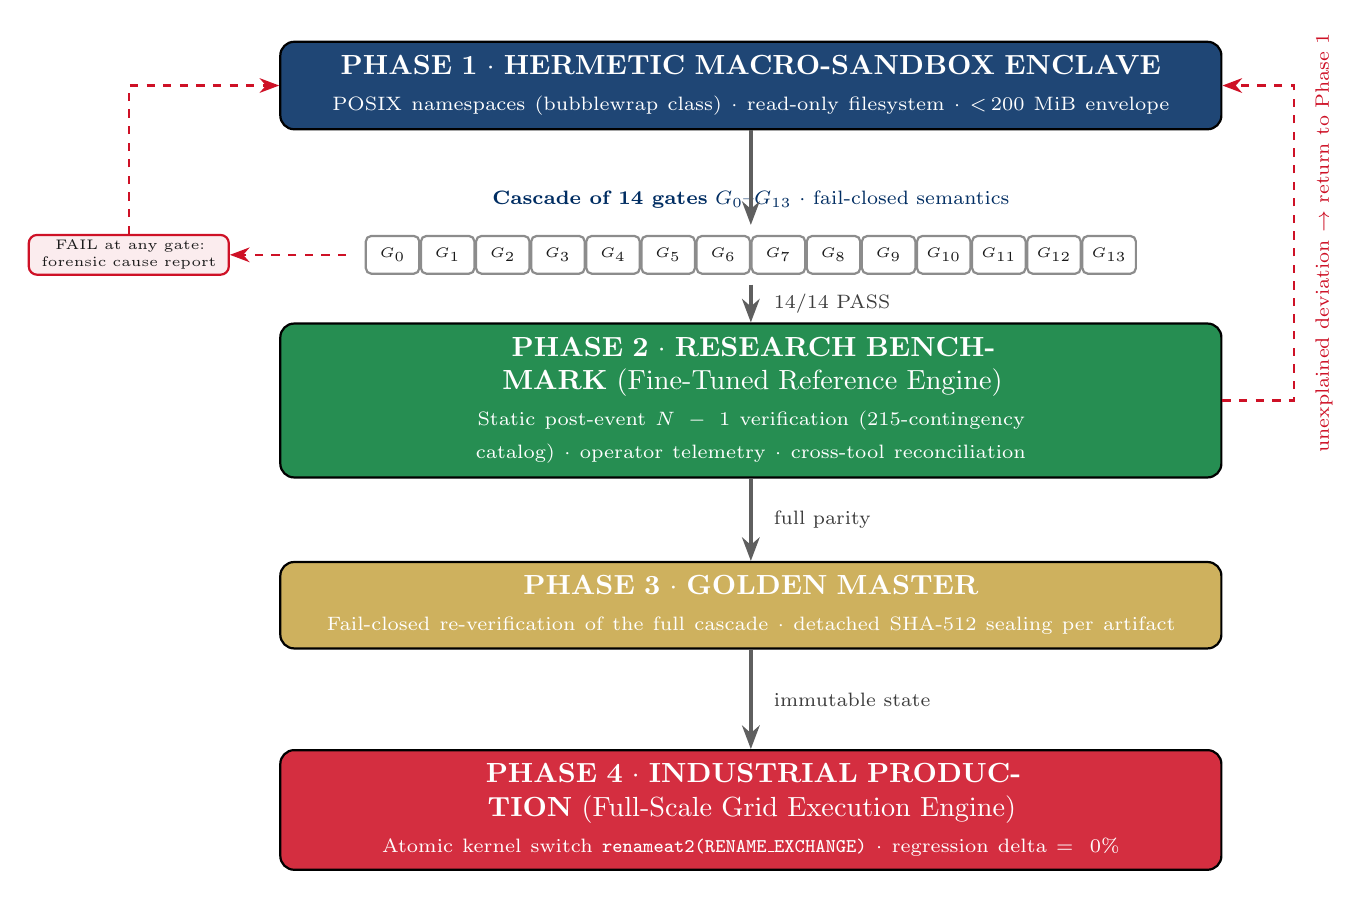
\begin{tikzpicture}[
  fase/.style={rectangle, rounded corners=5pt, draw, thick, text width=11.6cm, align=center, inner sep=5pt, minimum height=9mm},
  compuerta/.style={rectangle, rounded corners=2pt, draw=seni-dark!50, thick, fill=white, text=seni-dark, font=\tiny\bfseries, minimum width=6.8mm, minimum height=4.8mm, inner sep=0pt},
  forense/.style={rectangle, rounded corners=3pt, draw=seni-red, thick, fill=seni-red!8, text=seni-dark, font=\tiny, align=center, text width=2.4cm, inner sep=2pt},
  flujo/.style={-{Stealth[length=3mm]}, very thick, seni-dark!70},
  retorno/.style={-{Stealth[length=2.5mm]}, thick, seni-red, dashed},
  nota/.style={font=\scriptsize, text=seni-dark!85, align=center, fill=white, inner sep=2pt},
]
%% --- PHASE 1 ---
\node[fase, fill=seni-blue!88, text=white] (f1) at (0, 0) {
  \textbf{PHASE 1 $\cdot$ HERMETIC MACRO-SANDBOX ENCLAVE}\\[1pt]
  {\scriptsize POSIX namespaces (bubblewrap class) $\cdot$ read-only filesystem $\cdot$ ${<}\,200$ MiB envelope}
};
\node[nota, text=seni-blue] at (0, -1.45) {\textbf{Cascade of 14 gates} $G_0$--$G_{13}$ $\cdot$ fail-closed semantics};
%% --- Gates G0..G13 (single row) ---
\foreach \i in {0,...,13}{
  \node[compuerta] (g\i) at (-4.55+\i*0.70, -2.15) {$G_{\i}$};
}
%% --- PHASE 2 ---
\node[fase, fill=seni-green!85, text=white] (f2) at (0, -4.00) {
  \textbf{PHASE 2 $\cdot$ RESEARCH BENCHMARK} (Fine-Tuned Reference Engine)\\[1pt]
  {\scriptsize Static post-event $N-1$ verification (215-contingency catalog) $\cdot$ operator telemetry $\cdot$ cross-tool reconciliation}
};
%% --- PHASE 3 ---
\node[fase, fill=seni-gold!90, text=white] (f3) at (0, -6.60) {
  \textbf{PHASE 3 $\cdot$ GOLDEN MASTER}\\[1pt]
  {\scriptsize Fail-closed re-verification of the full cascade $\cdot$ detached SHA-512 sealing per artifact}
};
%% --- PHASE 4 ---
\node[fase, fill=seni-red!88, text=white] (f4) at (0, -9.20) {
  \textbf{PHASE 4 $\cdot$ INDUSTRIAL PRODUCTION} (Full-Scale Grid Execution Engine)\\[1pt]
  {\scriptsize Atomic kernel switch \texttt{renameat2(RENAME\_EXCHANGE)} $\cdot$ regression delta $= 0\%$}
};
%% --- Main flow (labels never crossed: midway white-filled) ---
\draw[flujo] (f1.south) -- (0, -1.77);
\draw[flujo] (0, -2.53) -- node[nota, right=2mm] {14/14 PASS} (f2.north);
\draw[flujo] (f2.south) -- node[nota, right=2mm] {full parity} (f3.north);
\draw[flujo] (f3.south) -- node[nota, right=2mm] {immutable state} (f4.north);
%% --- FAIL loop (left): forensic report and return to Phase 1 ---
\node[forense] (forense) at (-7.9, -2.15) {FAIL at any gate: forensic cause report};
\draw[retorno] (-5.14, -2.15) -- (forense.east);
\draw[retorno] (forense.north) -- (-7.9, 0) -- (f1.west);
%% --- Deviation loop (right): Phase 2 back to Phase 1 ---
\draw[retorno] (f2.east) -- (6.9, -4.00) -- (6.9, 0) -- (f1.east);
\node[nota, text=seni-red, rotate=90, align=center] at (7.28, -2.00) {unexplained deviation $\to$ return to Phase 1};
\end{tikzpicture}
} % extracted verbatim, sec01 L97--142
\caption{Cyber-physical four-phase digital-twin lifecycle with the fail-closed gate cascade. The Phase-1 hermetic enclave (POSIX namespaces, read-only filesystem, ${<}200$ MiB envelope) must pass the fourteen gates $G_0$--$G_{13}$ (14/14, fail-closed); the Phase-2 research testbed sustains static post-event $N-1$ verification against the 215-contingency catalog with operator telemetry and cross-tool reconciliation; the Phase-3 Golden Master is sealed with detached SHA-512 manifests; promotion to industrial production is an atomic kernel switch (renameat2, RENAME\_EXCHANGE) with zero regression. Any failed gate or unexplained deviation returns the package to Phase 1 with a forensic report: no intermediate states are admissible.}
\label{fig:gemelo_fases}
\end{figure*}


\subsection{SHA-512 cryptographic integrity digests}
\label{sub:seals}

Custody between stages is a chain of four SHA-512 seals. Each seal is detached from the stage that produced it and is checked by the stage that consumes it. Seal~1 closes intake (Ingesta): the screened commercial catalogs and the physical census. Seal~2 closes dispatch (Despacho): the merit-order schedule and the hourly injection series. Seal~3 closes the matrices and the forensic record (Matrices/Forense): the full admittance $\mathbf{Y}_{\mathrm{bus}}\in\mathbb{C}^{142\times 142}$, with its 20,164 complex entries and no ellipsis, and the unreduced polar Jacobian $\mathbf{J}\in\mathbb{R}^{282\times 282}$ in the four quadrants $\mathbf{J}_{P\theta}$, $\mathbf{J}_{PV}$, $\mathbf{J}_{Q\theta}$, $\mathbf{J}_{QV}$. Seal~4 closes the triad states (Estados Tríada): the real, ideal, and optimal operating points distinguished in Section~\ref{sub:triad}. A later stage accepts the previous stage only when the digest matches. A mismatch aborts the run.

Three certificates are issued from those seals.
\begin{enumerate}
\item \textbf{Certificate 1 --- convergence forensics.} It records the cascade that met the $10^{-8}$~pu stopping test, the final mismatch, and the identity of the method that accepted the state.
\item \textbf{Certificate 2 --- spectral integrity (SVD/Arnoldi).} It records $\kappa_2(\mathbf{J})=\sigma_{\max}/\sigma_{\min}$ from the singular-value decomposition and $\lambda_{\min}(\mathbf{J}_R)$ from the Arnoldi iteration of Section~\ref{sub:trinity}.
\item \textbf{Certificate 3 --- bit-for-bit kernel invariance.} It records that the deployed kernel and the sealed kernel are the same byte string, which is the custody hypothesis of Section~\ref{sub:lifecycle}.
\end{enumerate}

\subsection{Glass-box transparency}
\label{sub:glassbox}

An independent reader does not need the author's machine. The open structural arrays released with the benchmark on IEEE DataPort and the public repository --- the admittance matrices $\mathbf{Y}_{\mathrm{bus}}$ and the Jacobians, stored as \texttt{.npz} and \texttt{.json} --- are sufficient for the numerical replay. A validation script restricted to \texttt{numpy} and \texttt{scipy}, with no commercial power-system package, no PowerFactory and no PSS/E, replays the algebraic domain-decomposition residual of \eqref{eq:trinity},
\begin{equation*}
\|\mathbf{v}_{\mathrm{rec}}-\mathbf{v}_{\mathrm{full}}\|_\infty = 2.788 \times 10^{-14}\ \mathrm{pu} \le 10^{-11}\ \mathrm{pu},
\end{equation*}
and confirms the modal condition number $\kappa_2(\mathbf{J})$. The digits 2.788 are the residual already sealed in \eqref{eq:trinity}. The script is a replay, not a second measurement. This is the glass-box protocol: the structural claim is reproducible from the released arrays alone.

The release is split into two layers so that reproducibility of the network model is not confused with access to operational telemetry.
\begin{enumerate}
\item \textbf{Open Structural Benchmark (OSB).} The public deposit on IEEE DataPort and the public repository contains the 142-bus topology, the full branch parameters $R$, $X$, $B$, $S_{\max}$ and $I_{\max}$, the transformer parameters, the 69~kV reduction equivalents with the internal Joule loss assigned as $\Delta S_{\mathrm{loss}}$, and the canonical test cases of peak load, valley load, and maximum solar penetration.
\item \textbf{Operational Validation Bundle (OVB).} Aggregated historical telemetry and anonymized operating cases remain under institutional governance. They are the source of the decade used in Section~\ref{sub:dataprotocol}. They are not part of the open structural deposit.
\end{enumerate}

\subsection{Empirical data protocol}
\label{sub:dataprotocol}

The benchmark is not calibrated against assumptions; it is fed by an archived operational reality, and the protocol sentence is quoted verbatim as the contractual core of the data layer:
\begin{quote}
\itshape ``The structural solver is fed by a pre-existing, continuous empirical ground-truth repository comprising exactly 520 complete consecutive 168-hour weeks --- 87,360 hourly states over 3,640 Monday-to-Sunday days, selected without a single interpolated hour from the 2016--2025 operational archive --- provided by the Dominican Republic System Operator (Organismo Coordinador del SENI), capturing real SCADA telemetry, dispatch orders, solar/wind variable profiles, and historical outage logs.''
\end{quote}

Four variable families enter the solver from this repository: (i) nodal real and reactive demand at bulk buses; (ii) unit-by-unit dispatch of the thermal, hydro, solar, and wind fleet; (iii) meteorologically coupled solar and wind production profiles; and (iv) the historical outage log that seeds the contingency catalog. The validation horizon is standardized by construction: exactly 520 complete consecutive 168-hour weeks --- 87,360 hourly states over 3,640 Monday-to-Sunday days --- drawn from the 2016--2025 archive without a single interpolated hour. The civil span of the decade contains 3,653 days --- exactly 521 complete Monday-to-Sunday weeks (3,647 days, 87,528 hourly states) plus six calendar-boundary orphan days (January 1--3, 2016 and December 29--31, 2025). The standardized horizon adopts 520 of those 521 complete weeks --- Monday, January 4, 2016 through Sunday, December 21, 2025, i.e.\ 3,640 days or 87,360 hourly states --- so the thirteen excluded civil days decompose exactly into the six boundary orphan days plus the seven days of the final festive week (December 22--28, 2025), deliberately left out so that the atypical year-end collapse of industrial demand cannot contaminate the covariance structure of the block bootstrap. The exclusion is \emph{by construction}, not silent discarding. Retaining them would break the exact weekly periodicity of the archived dispatch and would truncate the resampling blocks at both ends: the 24-hour block bootstrap draws whole operating days aligned on the Monday-to-Sunday structure of the weekly generation, maintenance, and demand cycle, so week-complete selection guarantees that every draw is a physically realizable seven-day operating pattern and that no resampled block carries a truncation artifact of the civil calendar. Because the repository is continuous, the validation layer can resample it honestly: a \textbf{24-hour block bootstrap} draws whole operating days, preserving the intra-day correlation between irradiance, temperature, demand, and dispatch, rather than the decorrelated hour-level resampling that would flatter the error statistics of stability margins.

\subsection{Multi-temporal AC-OPF with power-to-gas coupling}
\label{sub:opf}

On the converged network model, the benchmark formulates a multi-temporal AC optimal power flow \cite{molzahn2019}. The dispatch prices energy and both reserve directions,
\begin{equation}
\min \sum_{t \in \mathcal{T}} \left[ \sum_{g \in \mathcal{G}} \left( c_g^{P}(P_{g,t}) + c_g^{+} r_{g,t}^{+} + c_g^{-} r_{g,t}^{-} \right) + \sum_{i \in \mathcal{V}} c^{\mathrm{shed}}\, P_{i,t}^{\mathrm{shed}} \right],
\label{eq:opfobj}
\end{equation}
subject to the AC balances, the thermal branch limits, the apparent-power disk \eqref{eq:capability}, the hourly ramps $|P_{g,t} - P_{g,t-1}| \le \Delta_g^{\mathrm{ramp}}$, and the storage balances of pumped hydro and hydrogen.

The shedding term is an exact penalty, not a modeling soft spot: the penalty $c^{\mathrm{shed}}$ is chosen strictly above any achievable system marginal cost, $c^{\mathrm{shed}} > \max_{g \in \mathcal{G}} \partial c_g^{P} / \partial P_{g,t}$. At an optimum, KKT stationarity in $P_{i,t}^{\mathrm{shed}}$ reads $c^{\mathrm{shed}} = \lambda_{i,t} + \mu_{i,t}$, with $\lambda_{i,t}$ the multiplier of the nodal balance \eqref{eq:opf_balance} and $\mu_{i,t} \ge 0$ the multiplier of the nonnegativity bound $P_{i,t}^{\mathrm{shed}} \ge 0$. Suppose unserved load were positive at optimality: complementarity would force $\mu_{i,t} = 0$ and hence $\lambda_{i,t} = c^{\mathrm{shed}}$. But whenever the post-event network is statically feasible, a shed-free dispatch exists, and the energy multiplier is then bounded by the marginal cost of the marginal committed unit, $\lambda_{i,t} \le \max_{g} \partial c_g^{P} / \partial P_{g,t} < c^{\mathrm{shed}}$ --- a contradiction. Optimality therefore carries $P_{\mathrm{shed}} = 0$ at every bus and hour in which the post-event network is statically feasible; clause 4 of the PASS battery of Section~\ref{sub:n1} is the verified instance of this structural property, not an assumption. The guarantee is quantitative under congestion: with the penalty fixed at the value of lost load, $c^{\mathrm{shed}} = 10{,}000\ \$/\mathrm{MWh}$, the highest registered marginal generation cost of the system below $230\ \$/\mathrm{MWh}$, and worst-case transmission-congestion rents not exceeding $120\ \$/\mathrm{MWh}$, the nodal energy multiplier is bounded by $\lambda_{i,t}^{\max} < 350\ \$/\mathrm{MWh}$; dual feasibility then gives $\mu_{i,t} = c^{\mathrm{shed}} - \lambda_{i,t} > 9{,}650 > 0$ strictly and uniformly under any admissible level of physical congestion, and complementarity forces $P_{i,t}^{\mathrm{shed}} = 0$ identically at every node where the network admits static feasibility.

For each hour $t$ and bus $i$, the equality constraints are the nodal balances, augmented with the power-to-gas coupling terms,
\begin{equation}
\sum_{g \in \mathcal{G}_i} P_{g,i,t} + \sum_{r \in \mathcal{R}_i} P_{r,i,t} + P_{i,t}^{\mathrm{FC}} - P_{i,t}^{\mathrm{EL}} + P_{i,t}^{\mathrm{shed}} - P_{i,t}^{\mathrm{load}} = P_i(\mathbf{V}_t, \boldsymbol{\theta}_t),
\label{eq:opf_balance}
\end{equation}
with the reactive analogue admitting inverter-coupled absorption/injection within apparent-power capability limits. The intertemporal coupling is imposed by the hydrogen buffer dynamics,
\begin{equation}
E_{h,t+1} = E_{h,t} + \left(\eta_{\mathrm{EL}}\, P_{h,t}^{\mathrm{EL}} - \frac{P_{h,t}^{\mathrm{FC}}}{\eta_{\mathrm{FC}}}\right) \Delta t, \qquad E_h^{\min} \le E_{h,t} \le E_h^{\max},
\label{eq:h2_storage}
\end{equation}
where $\eta_{\mathrm{EL}}$ and $\eta_{\mathrm{FC}}$ are the electrolysis and reconversion efficiencies: surplus non-dispatchable renewable generation becomes intertemporal energy inventory, absorbed as flexible electrolytic load in surplus hours and re-injected by the fuel cell in deficit hours. Pumped storage obeys the reservoir analogue with independent pump/turbine efficiencies, bounding the reversible 764~MW fleet of Section~\ref{sub:phes}. The complete problem is nonconvex because the AC equalities are nonconvex. It is solved by a cascade of thirty-two Newton-type configurations spanning Newton--Raphson \cite{tinney1967}, Iwamoto optimal-multiplier step control, fast-decoupled BX iterations \cite{stott1974}, and a Gauss--Seidel fallback, so that no single algebraic pathology can stall the sweep. The Karush--Kuhn--Tucker (KKT) system certifies local stationarity only. On this nonconvex problem the KKT conditions are necessary conditions at a local minimizer. They are not a certificate of global optimality. Stationarity of the Lagrangian, primal feasibility, dual feasibility, and complementarity are archived with the sealed validation output \cite{nocedal2006}, \cite{dommel1968}, \cite{wood2013}. Figure~\ref{fig:p2g_h2} diagrams the electrochemical coupling.

% ---- Figure 2 injection block (verbatim from the sealed master) ----
% Graphic source: sec02_modelado_matematico_ac_h2_sgen.tex, figure environment
% at L63--88 (styles: bloque/flujo/flujoh2/nota; palette seni-*).
% The tikzpicture is extracted verbatim from that source at injection time.
\begin{figure*}[!t]
\centering
\resizebox{0.85\textwidth}{!}{% Figure 2 tikzpicture — English edition (editorial refinement per
% GUIA_BUENAS_PRACTICAS_LATEX_IEEE: white-filled annotations, no line-through
% text; palette seni-* defined in the host preamble).
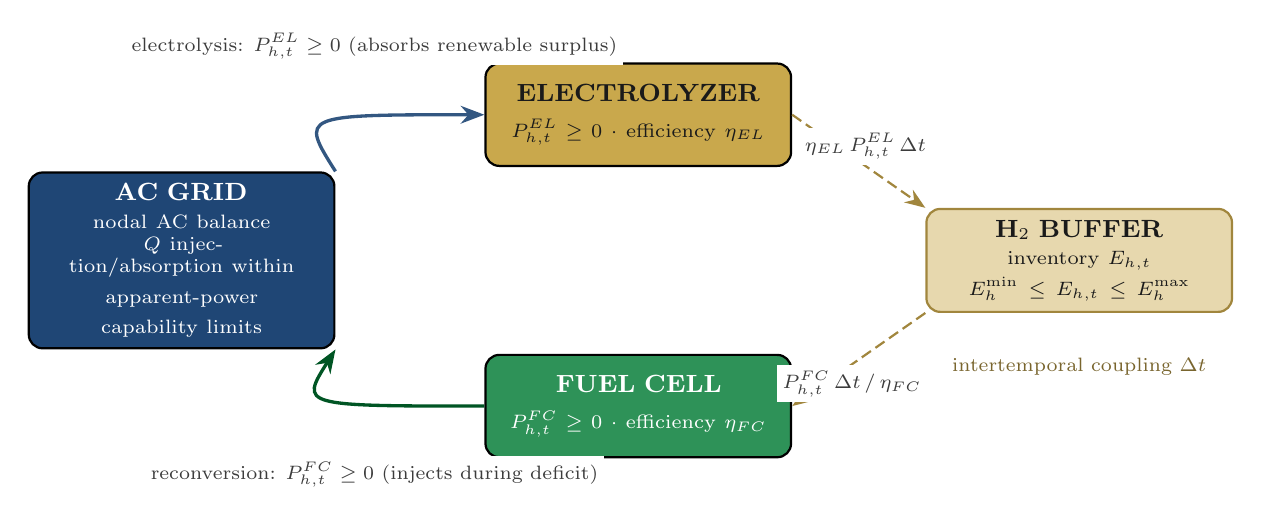
\begin{tikzpicture}[
  bloque/.style={rectangle, rounded corners=5pt, draw, thick, align=center, font=\small, text width=3.6cm, minimum height=13mm, inner sep=4pt},
  flujo/.style={-{Stealth[length=3mm]}, very thick},
  flujoh2/.style={-{Stealth[length=2.6mm]}, thick, seni-gold!80!black, dash pattern=on 4pt off 2pt},
  nota/.style={font=\scriptsize, align=center, text=seni-dark!85, fill=white, inner sep=2pt},
]
\node[bloque, fill=seni-blue!88, text=white] (red) at (0, 0) {\textbf{AC GRID}\\[2pt] {\scriptsize nodal AC balance\\$Q$ injection/absorption within\\apparent-power capability limits}};
\node[bloque, fill=seni-gold, text=seni-dark] (el) at (5.8, 1.85) {\textbf{ELECTROLYZER}\\[2pt] {\scriptsize $P^{EL}_{h,t} \ge 0$ $\cdot$ efficiency $\eta_{EL}$}};
\node[bloque, fill=seni-gold!45, draw=seni-gold!80!black, text=seni-dark] (buf) at (11.4, 0) {\textbf{H$_2$ BUFFER}\\[2pt] {\scriptsize inventory $E_{h,t}$\\$E^{\min}_h \le E_{h,t} \le E^{\max}_h$}};
\node[bloque, fill=seni-green!82, text=white] (fc) at (5.8, -1.85) {\textbf{FUEL CELL}\\[2pt] {\scriptsize $P^{FC}_{h,t} \ge 0$ $\cdot$ efficiency $\eta_{FC}$}};
%% --- Electric flows: grid <-> converters ---
\draw[flujo, seni-blue!80] (red.north east) .. controls (1.5,1.85) .. (el.west);
\node[nota] at (2.45, 2.72) {electrolysis: $P^{EL}_{h,t} \ge 0$ (absorbs renewable surplus)};
\draw[flujo, seni-green!70!black] (fc.west) .. controls (1.5,-1.85) .. (red.south east);
\node[nota] at (2.45, -2.72) {reconversion: $P^{FC}_{h,t} \ge 0$ (injects during deficit)};
%% --- Hydrogen flows: converters <-> buffer ---
\draw[flujoh2] (el.east) -- node[nota, above, pos=0.55] {$\eta_{EL}\, P^{EL}_{h,t}\, \Delta t$} (buf.north west);
\draw[flujoh2] (buf.south west) -- node[nota, below, pos=0.55] {$P^{FC}_{h,t}\, \Delta t\, /\, \eta_{FC}$} (fc.east);
%% --- Intertemporal coupling ---
\node[nota, text=seni-gold!60!black] at (11.4, -1.35) {intertemporal coupling $\Delta t$};
\end{tikzpicture}
} % extracted verbatim, sec02 L65--85
\caption{Electrochemical power-to-gas coupling of the green-hydrogen vector with the AC network. The electrolyzer absorbs renewable surplus as flexible load ($P^{\mathrm{EL}}_{h,t} \ge 0$, efficiency $\eta_{\mathrm{EL}}$); the storage buffer imposes the intertemporal inventory $E_{h,t+1} = E_{h,t} + (\eta_{\mathrm{EL}} P^{\mathrm{EL}}_{h,t} - P^{\mathrm{FC}}_{h,t}/\eta_{\mathrm{FC}})\,\Delta t$ with box constraints; the fuel cell re-injects power during deficit ($P^{\mathrm{FC}}_{h,t} \ge 0$, efficiency $\eta_{\mathrm{FC}}$). Both convertor terms enter the nodal AC balance. Electric flows in solid strokes; hydrogen flows in dashed gold.}
\label{fig:p2g_h2}
\end{figure*}


\subsection{Public doctrines of the diakoptic lifecycle}
\label{sub:doctrines}

The public doctrines below are the mathematical layer of the lifecycle that this benchmark executes. Each statement is an equation, not a narrative of implementation.

\textbf{Doctrine 01 --- border ports and Kron diakoptics.} Interior blocks are eliminated onto the cuts. The border operator is the Schur complement already factored in \eqref{eq:schur},
\begin{equation*}
S = D - C A^{-1} B.
\end{equation*}
Only the border ports remain as coupling variables.

\textbf{Doctrine 02 --- Th\'evenin/Norton preface and continuous Holter location.} While no retained bus is an island, the factorization $\mathbf{Y}=\mathbf{L}\mathbf{D}\mathbf{L}^{T}$ exists. The driving-point impedance at bus $i$ is the triangular solve $Z_{\mathrm{th},i}=\mathbf{e}_i^{T}\mathbf{Y}^{-1}\mathbf{e}_i$. A degree of zero, or a driving-point impedance that diverges, returns the component as an island. It does not return a Newton residual.

\textbf{Doctrine 03 --- soft-fail as a diagnosed deficit.} An infeasible balance is the exact-penalty problem
\begin{equation}
\min_{x,s}\ \tfrac12\lVert s\rVert^{2}\quad\mathrm{s.t.}\quad g(x)+s=0,
\label{eq:softfail}
\end{equation}
whose KKT stationarity identifies the deficit $s^{\star}=-\lambda^{\star}$. The slack variable is the certificate of the missing power. It is not a silent injection.

\textbf{Doctrine 04 --- substation and ring snapshots.} At iteration $t$ the supporting cut $\eta_k\ge\eta_k^{(t)}+\pi_k^{T}(v_c-v_c^{(t)})$ keeps a substation snapshot and a ring snapshot as valid outer approximations between solves.

\textbf{Doctrine 06 --- supervisors and cores decoupled by renewable source.} Fast electrical states $z$ and the port voltage $V$ separate by the singular perturbation $\varepsilon\dot{z}=f(z,V)$. The port map $(P,Q)=h(V)$ is what the master problem sees. Cores that face different renewable sources do not share an algebraic state.

\textbf{Doctrine 07 --- supervisors of on-load tap changers and SVCs.} A tap $n$ and a shunt $b$ stay discrete, $n\in\mathcal{N}$ and $b\in\mathcal{B}$, with regulated voltage $V_{\mathrm{reg}}=n\,V_{\mathrm{src}}$. The master accepts that discrete pair. It does not relax the tap into a fictitious continuous winding.

\textbf{Doctrine 09 --- continuous sigmoidal $Q$--$V$ regularization.} Renewable inverters use the odd sigmoidal map \eqref{eq:qsgen}. Its derivative enters $\mathbf{J}_{QV}$ and removes the PV--PQ chatter of Section~\ref{sub:regularization}.

\textbf{Doctrine 10 --- Kundur spectral supervisor.} The reduced reactive Jacobian is
\begin{equation}
\mathbf{J}_R = \mathbf{J}_{QV} - \mathbf{J}_{Q\theta}\, \mathbf{J}_{P\theta}^{-1}\, \mathbf{J}_{PV},
\label{eq:jr}
\end{equation}
and $\lambda_{\min}(\mathbf{J}_R)\to 0$ is the voltage-collapse test. It is not a restatement of $\kappa(\mathbf{J})$.

\textbf{Doctrine 11 --- HTLS reconductoring on the ideal network.} On $\mathcal{G}_{\mathrm{ideal}}$ a corridor is either kept or reconductored, $z_{\ell}\in\{0,1\}$. At the same sag, $I_{\mathrm{HTLS}}>I_{\mathrm{ACSR}}$. That thermal comparison is the statement used under CIGRE Technical Brochure 244.

\textbf{Doctrine 12 --- multiscale Th\'evenin/Norton reduction.} From the element up through the substation, the ring, and the national border, each eliminated interior obeys the Kron--Ward reduction
\begin{equation}
\mathbf{Y}_{\beta\beta}^{\mathrm{eq}} = \mathbf{Y}_{\beta\beta} - \mathbf{Y}_{\beta\alpha}\, \mathbf{Y}_{\alpha\alpha}^{-1}\, \mathbf{Y}_{\alpha\beta},
\label{eq:matrioshka}
\end{equation}
applied from the condensed 69~kV laterals onto the retained boundary terminals of Section~\ref{sub:reduction}, which stay at the measured 69~kV.

\textbf{Doctrine 14 --- territorial frontiers and the HBCF.} At a border port the Norton and Th\'evenin statements are $I_p=Y_p V_p+I_N$ and $V_p=Z_p I_p+E_{\mathrm{th}}$. Forward and backward sweeps meet at that port, and the block digest $h_e=\mathrm{SHA512}(\mathrm{canon}(\mathrm{block}))$ seals the frontier. The four macrodomains of Figure~\ref{fig:topologia142} are the electrical grouping of the Law 368-22 frontiers $\Gamma$.

\subsection{Topological reconciliation}
\label{sub:crosswalk}

Table~\ref{tab:crosswalk} states the census populations and the compute-model populations side by side. The two columns are different objects.

\begin{table}[!t]
\centering
\caption{Reconciliation of the physical census with the SENI-142 compute model.}
\label{tab:crosswalk}
\begin{tabular}{p{0.30\columnwidth}p{0.62\columnwidth}}
\toprule
Census object & Compute-model reading \\
\midrule
112 bulk transmission substations & fenced transmission estates at 345/230/138~kV hosting the compute model; distribution and medium-voltage yards are not instantiated \\
142 nodal compute buses & 115 bulk buses (6 at 345~kV, 3 at 230~kV, 106 at 138~kV) plus 27 condensed boundary ports at 69~kV \\
193 compute-model branches & 135 transmission lines and 58 power transformers, the complete released branch set of the benchmark \\
\bottomrule
\end{tabular}
\end{table}

The fourteen 138/69~kV transformer branches of Table~\ref{tab:cuadro51} feed those 27 boundary terminals. One estate can present several bays, a double busbar, or a three-winding unit that shares a single boundary interface, so the branch count and the terminal count are not equal. The 58 compute-model transformers remain the transformer edges inside the solved admittance. They are not the 68-branch winding inventory.

\subsection{Transmission-winding inventory and the reduced transport table}
\label{sub:inventory}

Table~\ref{tab:cuadro51} is the transmission-winding inventory: 68 branches whose two windings both sit at a transmission voltage. It is a different population from the 58 power transformers of the condensed compute model. Those 58 branches are the transformer edges that remain inside the solved 142-bus admittance. The 68 branches count every transmission-level winding pair in the estate survey, including the 34.5~kV secondary that Kron reduction removes from the nodal unknown.

\begin{table}[!t]
\centering
\caption{Transmission-winding inventory: 68 branches with both windings at transmission voltage. Shares are of this inventory.}
\label{tab:cuadro51}
\begin{tabular}{lrr}
\toprule
Winding pair & Branches & Share \\
\midrule
138/34.5~kV & 40 & 58.8\% \\
138/69~kV & 14 & 20.6\% \\
69/34.5~kV & 7 & 10.3\% \\
230/34.5~kV & 3 & 4.4\% \\
345/138~kV & 2 & 2.9\% \\
345/230~kV & 1 & 1.5\% \\
230/138~kV & 1 & 1.5\% \\
\midrule
Total & 68 & 100\% \\
\bottomrule
\end{tabular}
\end{table}

Power enters on the 345~kV corridors --- Punta Catalina, Julio Sauri, Bonao, Guerra, and the northern Manzanillo--El Naranjo circuit --- and is relieved downward. The two 345/138~kV branches (2.9\%) and the single 345/230~kV branch (1.5\%) are the step-down paths off the 345~kV backbone, so the loss of either path moves the undelivered corridor flow onto the surviving step. The 230~kV layer is thin: one 230/138~kV branch (1.5\%) and three 230/34.5~kV branches (4.4\%) absorb the Quisqueya and Pueblo Viejo injections into the 138~kV trunk or into local delivery. Absorption of load occurs on the 138~kV trunk. Forty 138/34.5~kV branches, 58.8\% of the inventory, deliver most of the power into distribution, and fourteen 138/69~kV branches (20.6\%) feed the retained boundary ports drawn in Figure~\ref{fig:topologia142}. The seven 69/34.5~kV branches (10.3\%) are the residual subtransmission delivery. Relief of a higher-voltage corridor is absorption at the next winding. It does not change the solved bus count. The share 58.8\% is the share of 138/34.5~kV branches inside these 68 branches.

Table~\ref{tab:buses142} lists the 115 named bulk yards at their measured nominal voltage, restricted to 345, 230, and 138~kV, with the Law 368-22 macrodomain of each yard. The solved cardinality is $142=115+27$. The 27 retained terminals are 69~kV ports of the 138/69~kV windings. They are drawn in Figure~\ref{fig:topologia142} and are not given a bulk voltage they do not have. Raw drawing coordinates do not appear.

% ---- Table: regional transactional balance (blindaje R3, EJE 3).
% Float sourced before tab:buses142 so that same-class float ordering lets it
% land on a text page in the two-column build instead of stranding at the flush. ----
\begin{table}[!t]
\centering
\caption{Regional Transactional Balance of the Four Macro-Domains (Law 368-22) at the Reference Peak State. Net interchanges close across the cut set $\Gamma$ ($\Sigma = 0$); internal network losses are embedded in the border injections of the exporting domains.}
\label{tab:regbalance}
\footnotesize
\setlength{\tabcolsep}{3pt}
\begin{tabular}{@{}lrrrl@{}}
\toprule
\textbf{Macro-domain} & \textbf{Dem.\ (MW)} & \textbf{Gen.\ (MW)} & \textbf{Net (MW)} & \textbf{Role} \\
\midrule
$\Omega_{\mathrm{Metro}}$ & 1,645 & 250 & $-1{,}395$ & Import hub \\
$\Omega_{\mathrm{Sur}}$ & 520 & 1,450 & $+930$ & Export \\
$\Omega_{\mathrm{Este}}$ & 680 & 1,100 & $+420$ & Export \\
$\Omega_{\mathrm{Norte}}$ & 605 & 650 & $+45$ & Local balance \\
\midrule
$\Sigma$ & 3,450 & 3,450 & $0$ & Balanced \\
\bottomrule
\end{tabular}
\end{table}

% Three-up transport table. Three logical columns, repeated. No raw coordinates.
\begin{table*}[!p]
\centering
\caption{Named bulk transport buses at the measured nominal voltage of 345, 230, or 138~kV (115 estates), ordered by macrodomain. The same three columns --- substation or bus, nominal kV, and Law 368-22 macrodomain or link corridor --- are repeated in three parallel groups so the inventory occupies one float page. The solved set has 142 nodes: these 115 yards plus 27 retained boundary terminals of the 138/69~kV windings, which keep their measured 69~kV and are drawn in Figure~\ref{fig:topologia142}. Raw drawing coordinates are omitted.}
\label{tab:buses142}
\resizebox{\textwidth}{!}{%
{\fontsize{6}{7}\selectfont
\setlength{\tabcolsep}{1.5pt}
\renewcommand{\arraystretch}{0.88}
\begin{tabular}{@{}lrl@{\hspace{3.5pt}}|@{\hspace{3.5pt}}lrl@{\hspace{3.5pt}}|@{\hspace{3.5pt}}lrl@{}}
\toprule
\textbf{Substation / bus} & \textbf{kV} & \textbf{Macrodomain / corridor} & \textbf{Substation / bus} & \textbf{kV} & \textbf{Macrodomain / corridor} & \textbf{Substation / bus} & \textbf{kV} & \textbf{Macrodomain / corridor} \\
\midrule
NAGUA 2 & 138 & \makecell[l]{$\Omega_1$ Norte\\Cibao Nordeste} & AGUACATE & 138 & \makecell[l]{$\Omega_2$ Sur\\Del Valle} & QUISQUEYA 2 & 230 & \makecell[l]{$\Omega_3$ Este\\Higuamo} \\
PAYITA & 138 & \makecell[l]{$\Omega_1$ Norte\\Cibao Nordeste} & PALOMINO & 138 & \makecell[l]{$\Omega_2$ Sur\\Del Valle} & SAN PEDRO BIOENERGY & 138 & \makecell[l]{$\Omega_3$ Este\\Higuamo} \\
PIMENTEL & 138 & \makecell[l]{$\Omega_1$ Norte\\Cibao Nordeste} & SAN JUAN 2 & 138 & \makecell[l]{$\Omega_2$ Sur\\Del Valle} & SIBA & 138 & \makecell[l]{$\Omega_3$ Este\\Higuamo} \\
PLAYA DORADA & 138 & \makecell[l]{$\Omega_1$ Norte\\Cibao Nordeste} & BARAHONA CARBON & 138 & \makecell[l]{$\Omega_2$ Sur\\Enriquillo} & SPM & 138 & \makecell[l]{$\Omega_3$ Este\\Higuamo} \\
PUERTO PLATA 2 & 138 & \makecell[l]{$\Omega_1$ Norte\\Cibao Nordeste} & CRUCE DE CABRAL 2 & 138 & \makecell[l]{$\Omega_2$ Sur\\Enriquillo} & SPM 2 & 138 & \makecell[l]{$\Omega_3$ Este\\Higuamo} \\
RIO SAN JUAN & 138 & \makecell[l]{$\Omega_1$ Norte\\Cibao Nordeste} & Jimaní & 138 & \makecell[l]{$\Omega_2$ Sur\\Enriquillo} & SULTANA DEL ESTE & 138 & \makecell[l]{$\Omega_3$ Este\\Higuamo} \\
S.F.M. & 138 & \makecell[l]{$\Omega_1$ Norte\\Cibao Nordeste} & LA GALLERA & 138 & \makecell[l]{$\Omega_2$ Sur\\Enriquillo} & CUMAYASA & 138 & \makecell[l]{$\Omega_3$ Este\\Yuma} \\
SALCEDO & 138 & \makecell[l]{$\Omega_1$ Norte\\Cibao Nordeste} & MATAFONGO & 138 & \makecell[l]{$\Omega_2$ Sur\\Enriquillo} & EL SEIBO & 138 & \makecell[l]{$\Omega_3$ Este\\Yuma} \\
SAN FELIPE & 138 & \makecell[l]{$\Omega_1$ Norte\\Cibao Nordeste} & PARAISO & 138 & \makecell[l]{$\Omega_2$ Sur\\Enriquillo} & EL SOCO & 138 & \makecell[l]{$\Omega_3$ Este\\Yuma} \\
Samaná & 138 & \makecell[l]{$\Omega_1$ Norte\\Cibao Nordeste} & PEDERNALES & 138 & \makecell[l]{$\Omega_2$ Sur\\Enriquillo} & Higüey & 138 & \makecell[l]{$\Omega_3$ Este\\Yuma} \\
Sánchez & 138 & \makecell[l]{$\Omega_1$ Norte\\Cibao Nordeste} & BAYASOL & 138 & \makecell[l]{$\Omega_2$ Sur\\Valdesia} & LA ROMANA & 138 & \makecell[l]{$\Omega_3$ Este\\Yuma} \\
AGUA CLARA & 138 & \makecell[l]{$\Omega_1$ Norte\\Cibao Noroeste} & CALABAZA & 138 & \makecell[l]{$\Omega_2$ Sur\\Valdesia} & MIRASOL & 138 & \makecell[l]{$\Omega_3$ Este\\Yuma} \\
Dajabón & 138 & \makecell[l]{$\Omega_1$ Norte\\Cibao Noroeste} & EL BRISAL & 138 & \makecell[l]{$\Omega_2$ Sur\\Valdesia} & ARROYO HONDO & 138 & \makecell[l]{$\Omega_4$ Metropolitano\\Ozama-Metropolitana} \\
ESPERANZA & 138 & \makecell[l]{$\Omega_1$ Norte\\Cibao Noroeste} & GUZMANCITO & 138 & \makecell[l]{$\Omega_2$ Sur\\Valdesia} & BOCA CHICA & 138 & \makecell[l]{$\Omega_4$ Metropolitano\\Ozama-Metropolitana} \\
GUANILLO & 138 & \makecell[l]{$\Omega_1$ Norte\\Cibao Noroeste} & ITABO & 138 & \makecell[l]{$\Omega_2$ Sur\\Valdesia} & CNP & 138 & \makecell[l]{$\Omega_4$ Metropolitano\\Ozama-Metropolitana} \\
GUAYUBIN & 138 & \makecell[l]{$\Omega_1$ Norte\\Cibao Noroeste} & ITABO TG & 138 & \makecell[l]{$\Omega_2$ Sur\\Valdesia} & DAJAO & 138 & \makecell[l]{$\Omega_4$ Metropolitano\\Ozama-Metropolitana} \\
LA ISABELA & 138 & \makecell[l]{$\Omega_1$ Norte\\Cibao Noroeste} & JIGUEY & 138 & \makecell[l]{$\Omega_2$ Sur\\Valdesia} & EMBAJADOR & 138 & \makecell[l]{$\Omega_4$ Metropolitano\\Ozama-Metropolitana} \\
MANZANILLO POWER LAND & 345 & \makecell[l]{$\Omega_1$ Norte\\Cibao Noroeste} & JULIO SAURI & 345 & \makecell[l]{$\Omega_2$ Sur\\Valdesia} & HAINA & 138 & \makecell[l]{$\Omega_4$ Metropolitano\\Ozama-Metropolitana} \\
MONTE CRISTI & 138 & \makecell[l]{$\Omega_1$ Norte\\Cibao Noroeste} & JULIO SAURI & 138 & \makecell[l]{$\Omega_2$ Sur\\Valdesia} & HAINAMOSA & 138 & \makecell[l]{$\Omega_4$ Metropolitano\\Ozama-Metropolitana} \\
Monción & 138 & \makecell[l]{$\Omega_1$ Norte\\Cibao Noroeste} & KM 15 DE AZUA & 138 & \makecell[l]{$\Omega_2$ Sur\\Valdesia} & HERRERA & 138 & \makecell[l]{$\Omega_4$ Metropolitano\\Ozama-Metropolitana} \\
SAJOMA & 138 & \makecell[l]{$\Omega_1$ Norte\\Cibao Noroeste} & MATRISOL & 138 & \makecell[l]{$\Omega_2$ Sur\\Valdesia} & LOS MINA & 138 & \makecell[l]{$\Omega_4$ Metropolitano\\Ozama-Metropolitana} \\
SANTIAGO RODRIGUEZ & 138 & \makecell[l]{$\Omega_1$ Norte\\Cibao Noroeste} & PALENQUE & 138 & \makecell[l]{$\Omega_2$ Sur\\Valdesia} & LOS MINA 5 & 138 & \makecell[l]{$\Omega_4$ Metropolitano\\Ozama-Metropolitana} \\
VALVERDE MAO & 138 & \makecell[l]{$\Omega_1$ Norte\\Cibao Noroeste} & PERAVIA & 138 & \makecell[l]{$\Omega_2$ Sur\\Valdesia} & LOS MINA 6 & 138 & \makecell[l]{$\Omega_4$ Metropolitano\\Ozama-Metropolitana} \\
CANABACOA & 138 & \makecell[l]{$\Omega_1$ Norte\\Cibao Norte} & PIZARRETE & 138 & \makecell[l]{$\Omega_2$ Sur\\Valdesia} & LOS MINA 7 & 138 & \makecell[l]{$\Omega_4$ Metropolitano\\Ozama-Metropolitana} \\
EL NARANJO & 345 & \makecell[l]{$\Omega_1$ Norte\\Cibao Norte} & PUNTA CATALINA & 345 & \makecell[l]{$\Omega_2$ Sur\\Valdesia} & LOS ORIGENES & 138 & \makecell[l]{$\Omega_4$ Metropolitano\\Ozama-Metropolitana} \\
EL NARANJO & 138 & \makecell[l]{$\Omega_1$ Norte\\Cibao Norte} & PUNTA CATALINA & 138 & \makecell[l]{$\Omega_2$ Sur\\Valdesia} & LOS PRADOS & 138 & \makecell[l]{$\Omega_4$ Metropolitano\\Ozama-Metropolitana} \\
LOPEZ ANGOSTURA & 138 & \makecell[l]{$\Omega_1$ Norte\\Cibao Norte} & SAN CRISTOBAL NORTE & 138 & \makecell[l]{$\Omega_2$ Sur\\Valdesia} & MATADERO & 138 & \makecell[l]{$\Omega_4$ Metropolitano\\Ozama-Metropolitana} \\
MOCA & 138 & \makecell[l]{$\Omega_1$ Norte\\Cibao Norte} & SANTANASOL & 138 & \makecell[l]{$\Omega_2$ Sur\\Valdesia} & METALDOM & 138 & \makecell[l]{$\Omega_4$ Metropolitano\\Ozama-Metropolitana} \\
NAVARRETE 2 & 138 & \makecell[l]{$\Omega_1$ Norte\\Cibao Norte} & VALDESIA & 138 & \makecell[l]{$\Omega_2$ Sur\\Valdesia} & METROPOLITANO & 138 & \makecell[l]{$\Omega_4$ Metropolitano\\Ozama-Metropolitana} \\
NIBAJE & 138 & \makecell[l]{$\Omega_1$ Norte\\Cibao Norte} & CIP LA LUISA & 138 & \makecell[l]{$\Omega_3$ Este\\Higuamo} & PALAMARA & 138 & \makecell[l]{$\Omega_4$ Metropolitano\\Ozama-Metropolitana} \\
TAVERA & 138 & \makecell[l]{$\Omega_1$ Norte\\Cibao Norte} & COASTAL & 138 & \makecell[l]{$\Omega_3$ Este\\Higuamo} & POWERSHIP KPS01 & 138 & \makecell[l]{$\Omega_4$ Metropolitano\\Ozama-Metropolitana} \\
ZF SANTIAGO & 138 & \makecell[l]{$\Omega_1$ Norte\\Cibao Norte} & ENERGAS 4 & 138 & \makecell[l]{$\Omega_3$ Este\\Higuamo} & POWERSHIP KPS26 & 138 & \makecell[l]{$\Omega_4$ Metropolitano\\Ozama-Metropolitana} \\
BONAO 2 & 138 & \makecell[l]{$\Omega_1$ Norte\\Cibao Sur} & GIRASOL & 138 & \makecell[l]{$\Omega_3$ Este\\Higuamo} & POWERSHIP KPS60 & 138 & \makecell[l]{$\Omega_4$ Metropolitano\\Ozama-Metropolitana} \\
BONAO 3 & 345 & \makecell[l]{$\Omega_1$ Norte\\Cibao Sur} & GUERRA & 345 & \makecell[l]{$\Omega_3$ Este\\Higuamo} & TIMBEQUE 2 & 138 & \makecell[l]{$\Omega_4$ Metropolitano\\Ozama-Metropolitana} \\
BONAO 3 & 138 & \makecell[l]{$\Omega_1$ Norte\\Cibao Sur} & GUERRA & 138 & \makecell[l]{$\Omega_3$ Este\\Higuamo} & UASD & 138 & \makecell[l]{$\Omega_4$ Metropolitano\\Ozama-Metropolitana} \\
COTOPERI & 138 & \makecell[l]{$\Omega_1$ Norte\\Cibao Sur} & HATO MAYOR 2 & 138 & \makecell[l]{$\Omega_3$ Este\\Higuamo} & VILLA DUARTE & 138 & \makecell[l]{$\Omega_4$ Metropolitano\\Ozama-Metropolitana} \\
FALCONDO & 138 & \makecell[l]{$\Omega_1$ Norte\\Cibao Sur} & JUAN DOLIO & 138 & \makecell[l]{$\Omega_3$ Este\\Higuamo} & VILLA MELLA & 138 & \makecell[l]{$\Omega_4$ Metropolitano\\Ozama-Metropolitana} \\
MONTE RIO & 138 & \makecell[l]{$\Omega_1$ Norte\\Cibao Sur} & MATA DE PALMA 2 & 138 & \makecell[l]{$\Omega_3$ Este\\Higuamo} &  & &  \\
PVDC & 230 & \makecell[l]{$\Omega_1$ Norte\\Cibao Sur} & QUISQUEYA 1 & 230 & \makecell[l]{$\Omega_3$ Este\\Higuamo} &  & &  \\
\bottomrule
\end{tabular}}}
\end{table*}

\subsection{The modular clause: instantiation under Law 368-22}
\label{sub:clause}

The invariant formulation binds itself to one reference reality by the following canonical closing clause, quoted verbatim:
\begin{quote}
\itshape ``In this reference benchmark, the structural payload is instantiated with the 142-bus insular bulk transmission grid of the Dominican Republic, partitioned into ten sovereign territorial microgrids under the legal framework of Spatial Planning and Land Use Law No. 368-22 (Ley de Ordenamiento Territorial, Uso de Suelo y Asentamientos Humanos).''
\end{quote}

The clause does three things at once. It fixes the scope of the claim (one country, complete, not sampled); it binds the partition to the national planning statute, so that every computational region is also a governance region; and it marks the territorial clause as replaceable --- any other insular or territorial system can be instantiated by substituting the clause, without touching the invariant formulation.


\bibliographystyle{IEEEtran}
\bibliography{referencias}

\end{document}
